\documentclass{bilidoc}

\geometry{
  a4paper,%
  left = 1.5cm,%
  right = 1.5cm,%
  top = 2.0cm,%
  bottom = 2.0cm%
}%

\usepackage{ulem}

\title{\textbf{\href{https://doi.org/10.1061/(ASCE)GT.1943-5606.0001206}{Static Liquefaction of Sands under Isotropically and $K_0$-Consolidated Undrained Triaxial Conditions }\\各向同性和$K_0$固结不排水三轴条件下砂土的静态液化}}

\author{Xilin Lu \thanks{
    Associate Professor, Dept. of Geotechnical Engineering and Key Laboratory of Geotechnical and Underground Engineering of the Ministry of Education, Tongji Univ., Shanghai 200092, China; formerly, Visiting Associate Professor, Dept. of Mechanical and Civil Engineering, California Institute of Technology, Pasadena, CA 91125 (corresponding author). E-mail: \url{xilinlu@tongji.edu.cn}.
} \and Maosong Huang \thanks{
    Professor and Chair, Dept. of Geotechnical Engineering and Key Laboratory of Geotechnical and Underground Engineering of the Ministry of Education, Tongji Univ., Shanghai 200092, China.
}}

\date{}

\begin{document}

\maketitle

\begin{Abstract}{Static liquefaction; Undrained triaxial tests; Critical state; Second-order work.}{静态液化; 不排水三轴试验; 临界状态; 二阶功。}

    By using the state-dependent strength criterion and dilatancy function, a state-dependent nonassociated elastoplasticity hardening model was proposed to unify modeling the constitutive relationships of sands with different initial void ratios. According to the second-order work theory, the criteria for predicting the potential instability and static liquefaction of sands were obtained. The proposed model and criteria were used to predict a series of isotropically consolidated and K0-consolidated undrained triaxial tests. The results showed that the potentially unstable point and the onset of static liquefaction under undrained conditions coincided with the attainment of a deviatoric stress peak in very loose sand, whereas, with the decrease of the initial void ratio, the onset of static liquefaction fell behind the potential instability. When the sand specimen was dense enough, static liquefaction did not occur, although the stress state was located inside of the potentially unstable region. The potential instability and static liquefaction occurred before the effective stress reached the failure surface, and they were the precursors though not the results of the sand failures.

    \switchcolumn

    利用状态相关的强度准则和剪胀函数,提出了状态相关的非关联弹塑性硬化模型,以统一建模具有不同初始孔隙率的砂土的本构关系。根据二阶功理论,获得了预测砂土潜在不稳定性和静态液化的标准。提出的模型和标准用于预测一系列各向同性固结和K0固结不排水三轴试验。结果表明,在不排水的条件下,潜在的不稳定点和静态液化的开始与在非常松散的砂土中获得的偏应力峰值相吻合,而随着初始孔隙率的降低,静态液化开始时间滞后于潜在失稳时间。当砂土样品足够致密时,尽管应力状态位于潜在不稳定区域的内部,但不会发生静态液化。在有效应力到达破坏面之前就发生了潜在的不稳定性和静态液化,尽管不是砂土破坏的结果,但它们是先兆。
    
\end{Abstract}

\begin{ParaColumn}[\bisection*{Introduction}{介绍}]

    The instability of soils that occurs before the peak failure often demonstrates as a localized or diffuse mode. The localized mode of instability appears in dense sand when loaded under drained condition, and it has been studied for a long time \citep{Rudnicki1975,Andrade2006,Lu2011}. For very loose sands, when monotonically loaded under an undrained condition, static liquefaction takes place; this kind of instability is different from the localized mode and keeps its homogeneous deformation. Static liquefaction is a typical and important characteristic of loosely compacted saturated soil, and it has been used in the stability analysis of saturated slope \citep{Lade1992,Ellison2009}.

    \switchcolumn

    在峰值破坏之前发生的土体不稳定性通常表现为局部或扩散模式。 在排水条件下加载时,局部失稳模式出现在稠密的沙子中,对此进行了长期的研究\citep{Rudnicki1975,Andrade2006,Lu2011}。 对于非常疏松的砂,在不排水的情况下单调加载时,会发生静态液化。 这种不稳定性不同于局部模式,并保持其均匀变形。 静态液化是松散压实的饱和土的典型和重要特征,已用于饱和边坡的稳定性分析\citep{Lade1992,Ellison2009}。

    \switchcolumn*

    Static liquefaction has been studied experimentally by triaxial tests \citep{Sladen1985, Lade1990,Yamamuro1997,Doanh1997}, plane-strain tests \citep{Chu2008}, and ring-shear tests \citep{Liu2011}. The influence of K0 consolidation on static liquefaction was also studied experimentally \citep{Fourie2005, Chu2008}. Based on the summary of existing experimental results, the onset of static liquefaction instability could be determined by the instability line \citep{Lade1990} or collapse surface \citep{Sladen1985} in stress space. The experimental results \citep{Daouadji2010,Wanatowski2012} showed the main factors affecting instability are the stress state, drainage condition, loading mode, and material state. By summing up a series of experimental results, the undrained instability has been characterized by critical state theory \citep{Rahman2011,Bedin2012}. To describe the influence of the initial material state on instability, \citet{Yang2002} expressed the instability line as a function of the current material state, and \citet{Rahman2011} defined the instability line as a function of the equivalent granular state parameter.

    \switchcolumn

    静态液化已通过三轴试验\citep{Sladen1985, Lade1990,Yamamuro1997,Doanh1997},平面应变试验\citep{Chu2008}和环刀剪切试验\citep{Liu2011}进行了实验研究。还通过实验研究了K0固结对静态液化的影响\citep{Fourie2005, Chu2008}。根据现有实验结果的总结,静态液化不稳定性的发生可以通过应力空间中的不稳定性线\citep{Lade1990}或坍塌表面\citep{Sladen1985}来确定。实验结果\citep{Daouadji2010,Wanatowski2012}表明,影响失稳的主要因素是应力状态,排水条件,加载模式和材料状态。通过总结一系列实验结果,通过临界状态理论对不排水的不稳定性进行了表征\citep{Rahman2011,Bedin2012}。为了描述初始材料状态对不稳定性的影响,\citet{Yang2002}将不稳定性线表示为当前材料状态的函数,\citet{Rahman2011}将不稳定性线定义为等效颗粒状态参数的函数。

    \switchcolumn*

    Compared with the experimental studies, there is lack of theoretical study on static liquefaction. \citet{Borja2006} adopted the bifurcation theory to study the initiation of liquefaction instability in saturated soils. \citet{Andrade2009} presented a practical mathematical framework for predicting the liquefaction instability, which has been shown to coincide with the loss of uniqueness of material response \citep{Nova1994}. \citet{Buscarnera2011} studied diffuse instability by loss of controllability and derived the mathematical condition under different loading conditions. Based on the Nor-Sand model \citep{Jefferies1993, Andrade2008}, the critical hardening modulus corresponding to the onset of static liquefaction was obtained and adopted in numerical modeling of submarine slope \citep{Ellison2009}. In these works, static liquefaction was predicted to occur at the strain-softening stage; instability can also emerge within stable single-phase solids owing to the interaction between the solid matrix and fluid flow \citep{Bardet2002}.

    \switchcolumn

    与实验研究相比,缺乏关于静态液化的理论研究。 \citet{Borja2006}运用分叉理论研究了饱和土壤中液化不稳定性的起因。 \citet{Andrade2009}提出了一个实用的数学框架来预测液化不稳定性,这已经证明与材料响应唯一性的丧失相吻合\citep{Nova1994}。\citet{Buscarnera2011}研究了由于失控引起的扩散不稳定性,并推导了不同载荷条件下的数学条件。基于Nor-Sand模型\citep{Jefferies1993, Andrade2008},获得了对应于静态液化开始的临界硬化模量,并将其用于海底边坡的数值模拟中\citep{Ellison2009}。在这些工作中,预计在应变软化阶段会发生静态液化。由于固体基质和流体之间的相互作用,在稳定的单相固体中也可能出现不稳定性\citep{Bardet2002}。

    \switchcolumn*

    This paper proposes a model to calibrate the stress-strain relationships and study the onset of static liquefaction under different initial material states, consolidation states, and confining conditions. After a view of the critical state theory, a state-dependent Mohr-Coulomb elastoplasticity hardening model is proposed by using material state–dependent strength and stress dilatancy. Based on the second-order work criterion, the theoretical condition for static liquefaction is proposed and used to predict the results of isotropically consolidated and $K_0$-consolidated undrained triaxial compression tests. Finally, the influence of the initial material states of sands at the onset of static liquefaction is discussed.

    \switchcolumn

    本文提出了一个校准应力-应变关系的模型,并研究了在不同初始材料状态,固结状态和约束条件下静态液化的开始。 根据临界状态理论,通过使用材料状态相关的强度和应力膨胀率,提出了状态相关的摩尔库伦弹塑性硬化模型。 基于二阶功准则,提出了静态液化的理论条件,并将其用于各向同性固结和$K_0$固结不排水三轴压缩试验的结果。 最后,讨论了砂土初始材料状态在静态液化开始时的影响。

\end{ParaColumn}
\begin{ParaColumn}[\bisection*{State-Dependent Elastoplasticity Model: Critical State Theory}{状态相关的弹塑性模型:临界状态理论}]
    
    The state parameter $\psi$ \citep{Been1985}, which represents the difference of current void ratio $e$ and the void ratio $e_c$ at the critical state in the same mean pressure, can be used to determine the state of soil

    \switchcolumn

    状态参数$\psi$ \citep{Been1985}表示在相同平均压力下临界状态下当前空隙率$e$和空隙率$e_c$之差,可用于确定土体状态

    \CrossColumnText{
        \begin{align}
            \psi=e-e_{c}
        \end{align}
    }
    \switchcolumn*

    \noindent
    The void ratio ec at the critical state line depends on the mean pressure; it can be defined by \citep{Yang2004}

    \switchcolumn

    \noindent
    临界状态线处的空隙率$e_c$取决于平均压力。 它可以定义为\citep{Yang2004}

    \CrossColumnText{
        \begin{align}
            e_{c}=e_{c 0}-\lambda_{c}\left(\frac{p}{p_{a t}}\right)^{\xi}
        \end{align}
    }
    \switchcolumn*

    \noindent
    where $p_{a t}=101.3 \mathrm{kPa}$ = atmospheric pressure; and $e_{c 0}, \lambda_{c},$ and $\xi=$ material parameters that are used to determine the critical state line in the $e, p$-plane.

    \switchcolumn

    \noindent
    其中$p_{a t}=101.3 \mathrm{kPa}$为大气压力;$e_{c 0}, \lambda_{c},$和$\xi=$为材料参数,这些材料参数用于确定$e,p$平面中的临界状态线。

    \switchcolumn*

    In \enautoref{figure:1}, the state parameter $\psi$ clearly shows the state of the sand; a negative value indicates dilative state and a positive value indicates contractive state. It should be noted that, in an undrained case, the total volumetric strain always keeps constant, and the attainment of the state parameter to the critical state is caused by the changes in the effective mean pressure.

    \switchcolumn

    在\cnautoref{figure:1}中,状态参数$\psi$清楚地显示了砂土的状态。 负值表示扩张状态,正值表示收缩状态。 应该注意的是,在不排水的情况下,总体积应变始终保持恒定,并且状态参数达到临界状态是由有效平均压力的变化引起的。

    \CrossColumnText{
        \begin{figure}[htb]
    \centering
    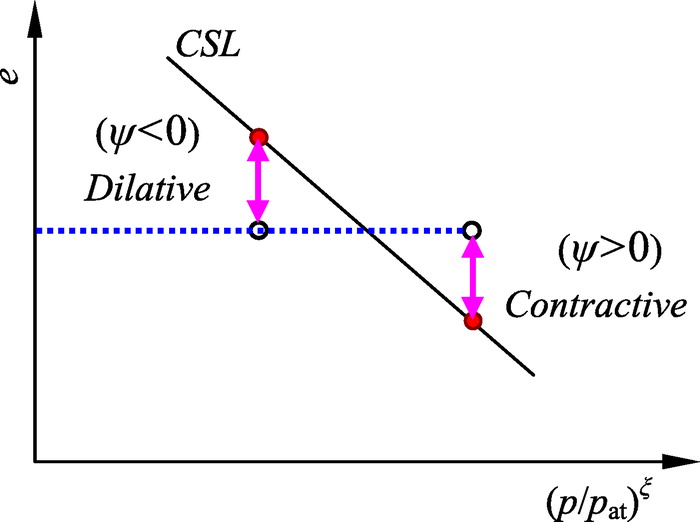
\includegraphics[width=.5\textwidth]{figures/figure1.jpg}
    \bicaption{Critical state line in $e-\left(p / p_{a t}\right)^{\xi}$ plane}{$e-\left(p / p_{a t}\right)^{\xi}$平面的临界状态线}
    \label{figure:1}
\end{figure}
    }

\end{ParaColumn}
\begin{ParaColumn}[\bisection*{State-Dependent Mohr-Coulomb Hardening Model}{状态相关的摩尔库伦硬化模型}]
    
    Considering the theoretical prediction of the onset of static liquefaction relies on the constitutive relationships, a sophisticated model needs to be developed to capture the instability characteristic of the sands with different initial material states. Here, for simplicity, the constitutive model is proposed on the basis of the widely used elastoplastic Mohr-Coulomb hardening model. The yield function is
    
    \switchcolumn

    考虑到静态液化开始的理论预测依赖于本构关系,需要建立一个复杂的模型来捕捉不同初始物质状态的砂土的失稳特性。为简便起见,在广泛应用的摩尔-库仑强化模型的基础上,提出了本构模型。屈服函数为

    \CrossColumnText{
        \begin{align}
            F=q-M p^{\prime}=0
            \label{equation:3}
        \end{align}
    }
    \switchcolumn*

    \noindent
    where $p^{\prime}=\sigma_{i i} / 3-u$; $q=\sqrt{3 J_{2}}=\sqrt{3 s_{i j}^{\prime} s_{i j}^{\prime} / 2}$; $s_{i j}^{\prime}=\boldsymbol{\sigma}_{i j}^{\prime}-\delta_{i j} p^{\prime}$; $\boldsymbol{\sigma}_{i j}^{\prime}=\boldsymbol{\sigma}_{i j}-u$; $u=$ pore-water pressure; and $\delta_{i j}=$ Kronecker delta.

    \switchcolumn

    \noindent
    其中$p^{\prime}=\sigma_{i i} / 3-u$;$q=\sqrt{3 J_{2}}=\sqrt{3 s_{i j}^{\prime} s_{i j}^{\prime} / 2}$;$s_{i j}^{\prime}=\boldsymbol{\sigma}_{i j}^{\prime}-\delta_{i j} p^{\prime}$; $\boldsymbol{\sigma}_{i j}^{\prime}=\boldsymbol{\sigma}_{i j}-u$;$u$为孔隙水压力,$\delta_{i j}$为克罗内克符号。

    \switchcolumn*

    The evolution of $M$ is assumed to follow the hyperbolic law \citep{Pietruszczak1987,Huang2010}

    \switchcolumn

    假设$M$的演化遵循双曲线规律\citep{Pietruszczak1987,Huang2010}

    \CrossColumnText{
        \begin{align}
            M=M_{p} \frac{\varepsilon_{s}^{p}}{A+\varepsilon_{s}^{p}}
        \end{align}
    }
    \switchcolumn*

    \noindent
    where the equivalent plastic shear strain $\varepsilon_{s}^{p}=\sqrt{2 e_{i j} e_{i j} / 3}$; $e_{i j}=\varepsilon_{i j}-\delta_{i j} \varepsilon_{i i}/3$ and $A=$ fitting parameter. The peak value of stress ratio $M_{p}$ is assumed to be state-dependent and can be expressed as \citep{Manzari1997}

    \switchcolumn

    \noindent
    其中等效塑性剪切应变$\varepsilon_{s}^{p}=\sqrt{2 e_{i j} e_{i j} / 3}$;$e_{i j}=\varepsilon_{i j}-\delta_{i j} \varepsilon_{i i}/3$以及$A$为拟合参数。 假定应力比$M_{p}$的峰值与状态有关,可以表示为\citep{Manzari1997}

    \CrossColumnText{
        \begin{align}
            M_{p}=M_{c s} \exp \left(-n^{b} \psi\right)
            \label{equation:5}
        \end{align}
    }
    \switchcolumn*

    The plastic dilatancy is

    \switchcolumn
    
    塑性剪胀为

    \CrossColumnText{
        \begin{align}
            D=\frac{d \varepsilon_{v}^{p}}{d \varepsilon_{s}^{p}}
        \end{align}
    }
    \switchcolumn*

    \noindent
    A framework is needed to define a unique relationship between the stress ratio and the dilatancy. To capture the influence of the material state, the state parameter should be included in the stress-dilatancy function, and it could be formulated as \citep{Li2000,Gajo2001}

    \switchcolumn

    \noindent
    需要一个框架来定义应力比和膨胀率之间的唯一关系。 为了捕获物质状态的影响,应将状态参数包括在应力剪胀函数中,并且可以将其表达为\citep{Li2000,Gajo2001}。

    \CrossColumnText{
        \begin{align}
            D=A_{d}\left[M_{d}-M\right]=A_{d}\left[M_{c s} \exp \left(n^{d} \psi\right)-M\right]
            \label{equation:7}
        \end{align}
    }
    \switchcolumn*

    \noindent
    where $A_{d}=d_{0} / M_{c s}$; and $n^{d}$ and $d_{0}$ = material parameters.

    \switchcolumn

    \noindent
    式中$A_{d}=d_{0} / M_{c s}$;$n^{d}$和$d_{0}$为材料常数。

    \switchcolumn*

    For simplicity, here Ad is assumed to be 1, and then \enautoref{equation:7} is the same for the dilatancy function in the Cam-clay model and can be formulated equivalently by using the plastic potential function

    \switchcolumn

    为简单起见,此处假设$A_d$为1,然后对于剑桥粘土模型中的剪胀函数,\cnautoref{equation:7}相同,并且可以使用塑性势函数等效地公式化

    \CrossColumnText{
        \begin{align}
            G=q+M_{d} p^{\prime} \ln \frac{p^{\prime}}{p_{0}}=0
            \label{equation:8}
        \end{align}
    }
    \switchcolumn*

    \noindent
    From Eqs. \ref{equation:3} and \ref{equation:8}, the gradient of yield function and plastic potential function to $p^\prime$ and $q$ are

    \switchcolumn

    \noindent
    由\cnautoref{equation:3}和\cnautoref{equation:8},屈服函数和塑性势函数到$p^\prime$和$q$的梯度为

    \CrossColumnText{
        \begin{align}
            \begin{aligned}
                \frac{\partial F}{\partial p^{\prime}}&=-M \\
                \frac{\partial F}{\partial q}&=1\\
            \end{aligned}
            \label{equation:9}
        \end{align}

        \begin{align}
            \begin{aligned}
                \frac{\partial Q}{\partial p^{\prime}}&=M_{d}-\frac{q}{p^{\prime}} \\
                \frac{\partial Q}{\partial q}&=1
            \end{aligned}
            \label{equation:10}
        \end{align}
    }
    \switchcolumn*

    The rate form of elastoplasticity constitutive relationship is

    \switchcolumn

    弹塑性本构关系的速率形式为

    \CrossColumnText{
        \begin{align}
            \dot{\sigma}_{i j}=\mathbf{D}_{i j k l}^{e p} \dot{\varepsilon}_{k l}
            \label{equation:11}
        \end{align}
    }
    \switchcolumn*

    \noindent
    where the elastoplastic modulus is

    \switchcolumn

    \noindent
    弹塑性模量为

    \CrossColumnText{
        \begin{align}
            \begin{aligned}
                \mathbf{D}_{i j k l}^{e p}=\mathbf{D}_{i j k l}^{e}-\mathbf{D}_{i j k l}^{p}=&\left(K-\frac{2}{3} G\right) \delta_{i j} \delta_{k l}+G\left(\delta_{i k} \delta_{j l}+\delta_{i l} \delta_{j k}\right) \\
                &-\dfrac{D_{i j m n}^{e} \dfrac{\partial Q}{\partial \sigma_{m n}^{\prime}}\left(\dfrac{\partial F}{\partial \sigma_{p q}^{\prime}}\right)^{T} D_{p q k l}^{e}}{\left(\dfrac{\partial F}{\partial \sigma_{u v}^{\prime}}\right)^{T} D_{u v s t}^{e} \dfrac{\partial Q}{\partial \sigma_{s t}^{\prime}}+H_{p}}
        \end{aligned}
        \end{align}
    }
    \switchcolumn*

    \noindent
    The hardening modulus is

    \switchcolumn

    \noindent
    硬化模量为

    \CrossColumnText{
        \begin{align}
            H_{p}=-\frac{\partial F}{\partial M} \frac{\partial M}{\partial \varepsilon_{s}^{p}}=p^{\prime} M_{p} \frac{A}{\left(A+\varepsilon_{e p}\right)^{2}}
        \end{align}
    }
    \switchcolumn*

    The bulk modulus K and shear modulus G are related to the state of sand and can be expressed by the current void ratio e as \citep{ERichart1970}

    \switchcolumn

    体积模量$K$和剪切模量$G$与砂的状态有关,可以用当前的孔隙率$e$表示为\citep{ERichart1970}

    \CrossColumnText{
        \begin{align}
            \begin{aligned}
            K&=\frac{2(1+\nu)}{3(1-2 \nu)} G \\
            G&=G_{0} p_{a t} \frac{(2.97-e)^{2}}{1+e} \sqrt{\frac{p^{\prime}}{p_{a t}}}
            \end{aligned}
            \label{equation:14}
        \end{align}
    }
    \switchcolumn*

    \noindent
    where $G_0$ = regression constant of the elastic shear modulus; and $\nu$ = Poisson’s ratio.

    \switchcolumn

    \noindent
    其中$G_0$为弹性剪切模量的回归常数;$\nu$为泊松比。
\end{ParaColumn}
\begin{ParaColumn}[\bisection*{$p-q$ Form under Triaxial Condition}{三轴条件下的$p-q$形式}]
    
    To simulate the stress-strain relationship of soil under the triaxial condition conveniently, \enautoref{equation:11} is rewritten into $p-q$ form as

    \switchcolumn

    为了方便地模拟三轴条件下土体的应力-应变关系,可将\cnautoref{equation:11}被重写为$p-q$形式为

    \CrossColumnText{
        \begin{align}
            \begin{aligned}
            \dot{p}^{\prime}=K \dot{\varepsilon}_{v}^{e}=K\left(\dot{\varepsilon}_{v}-\dot{\lambda} \frac{\partial Q}{\partial p^{\prime}}\right) \\
            \dot{q}=3 G \dot{\varepsilon}_{s}^{e}=3 G\left(\dot{\varepsilon}_{s}-\dot{\lambda} \frac{\partial Q}{\partial q}\right)
            \end{aligned}
            \label{equation:15}
        \end{align}
    }
    \switchcolumn*

    \noindent
    where $\varepsilon_{s}=2\left(\varepsilon_{a}-\varepsilon_{r}\right) / 3$; $\varepsilon_{v}=2 \varepsilon_{a}+\varepsilon_{r}$; $p^{\prime}=\left(\sigma_{a}^{\prime}+2 \sigma_{r}^{\prime}\right) / 3$; $q=\sigma_{a}^{\prime}-\sigma_{r}^{\prime}$; $\varepsilon_{a}$ and $\varepsilon_{r}=$ axial and radial strains; and $\sigma_{a}^{\prime}$ and $\sigma_{r}^{\prime}=$ axial and radial effective stresses.

    \switchcolumn

    \noindent
    式中$\varepsilon_{s}=2\left(\varepsilon_{a}-\varepsilon_{r}\right) / 3$; $\varepsilon_{v}=2 \varepsilon_{a}+\varepsilon_{r}$; $p^{\prime}=\left(\sigma_{a}^{\prime}+2 \sigma_{r}^{\prime}\right) / 3$; $q=\sigma_{a}^{\prime}-\sigma_{r}^{\prime}$; $\varepsilon_{a}$和$\varepsilon_{r}$为轴向和径向应变;$\sigma_{a}^{\prime}$和$\sigma_{r}^{\prime}$为轴向和径向有效应力。

    \switchcolumn*

    The plastic multiplier could be obtained from the consistency condition and can be expressed as

    \switchcolumn

    可从一致性条件获得塑性乘数,并表示为

    \CrossColumnText{
        \begin{align}
            \dot{\lambda}=\frac{K \dfrac{\partial F}{\partial p^{\prime}} \dot{\varepsilon}_{v}+3 G \dfrac{\partial F}{\partial q} \dot{\varepsilon}_{s}}{H_{p}+K \dfrac{\partial F}{\partial p^{\prime}} \dfrac{\partial Q}{\partial p^{\prime}}+3 G \dfrac{\partial F}{\partial q} \dfrac{\partial Q}{\partial q}}
            \label{equation:16}
        \end{align}
    }
    \switchcolumn*

    \noindent
    Using Eqs. \ref{equation:9} and \ref{equation:10}, \enautoref{equation:16} becomes

    \switchcolumn

    \noindent
    联立\cnautoref{equation:9}和\cnautoref{equation:10},\cnautoref{equation:16}变为

    \CrossColumnText{
        \begin{align}
            \dot{\lambda}=\frac{-K M \dot{\varepsilon}_{v}+3 G \dot{\varepsilon}_{s}}{H_{p}+K M\left(M-M_{d}\right)+3 G}
        \end{align}
    }
    \switchcolumn*

    The deviatoric and volumetric plastic strain rates are

    \switchcolumn

    变形和体积塑性应变率分别为

    \CrossColumnText{
        \begin{align}
            \begin{array}{c}
            \dot{\varepsilon}_{v}^{p}=\dot{\lambda} \dfrac{\partial Q}{\partial p^{\prime}}=\dot{\lambda} M_{d}\left(\ln \dfrac{p^{\prime}}{p_{0}}+1\right)=\dot{\lambda}\left(M_{d}-M\right) \\
            \dot{\varepsilon}_{s}^{p}=\dot{\lambda} \dfrac{\partial Q}{\partial q}=\dot{\lambda}
            \end{array}
            \label{equation:18}
        \end{align}
    }
    \switchcolumn*

    \noindent
    By inserting \enautoref{equation:18} into \enautoref{equation:18}, one gets

    \switchcolumn

    \noindent
    将\cnautoref{equation:18}代入\cnautoref{equation:15},得到

    \CrossColumnText{
        \begin{align}
            \begin{array}{c}
            \dot{p}^{\prime}=K\left[\dot{\varepsilon}_{v}-\dot{\lambda}\left(M_{d}-M\right)\right] \\
            \dot{q}=3 G\left(\dot{\varepsilon}_{s}-\dot{\lambda}\right)
            \end{array}
        \end{align}
    }

    \switchcolumn*

    After arrangement, the rate form of the constitutive relationship is

    \switchcolumn

    整理后,本构关系的比率形式为

    \CrossColumnText{
        \begin{align}
            \left\{\begin{array}{c}
            \dot{p}^{\prime} \\
            \dot{q}
            \end{array}\right\}=\mathbf{D}_{p q}^{e p}\left\{\begin{array}{l}
            \dot{\varepsilon}_{v} \\
            \dot{\varepsilon}_{s}
            \end{array}\right\}
            \label{equation:20}
        \end{align}
    }
    \switchcolumn*

    \noindent
    where

    \switchcolumn

    \noindent
    式中

    \CrossColumnText{
        \begin{align*}
            \mathbf{D}_{p q}^{e p}=\left[\begin{array}{cc}
            K+\dfrac{K^{2} M\left(M_{d}-M\right)}{H_{p}+K M\left(M-M_{d}\right)+3 G} & \dfrac{-3 K G\left(M_{d}-M\right)}{H_{p}+K M\left(M-M_{d}\right)+3 G} \\
            \dfrac{3 K G M}{H_{p}+K M\left(M-M_{d}\right)+3 G} & 3 G-\dfrac{9 G^{2}}{H_{p}+K M\left(M-M_{d}\right)+3 G}
            \end{array}\right]
        \end{align*}
    }
\end{ParaColumn}
\begin{ParaColumn}[\bisection*{$K_0$-Consolidated Condition}{$K_0$固结状态}]
    
    When the state-dependent Mohr-Coulomb hardening model was used to simulate the $K0$-consolidated undrained triaxial tests, the evolution of $M$ needed to be changed as

    \switchcolumn

    当使用状态依赖的摩尔库伦硬化模型来模拟$K_0$固结不排水三轴试验时,$M$的演变需要更改为

    \CrossColumnText{
        \begin{align}
            M=M_{0}+\left(M_{p}-M_{0}\right) \frac{\varepsilon_{s}^{p}}{A+\varepsilon_{s}^{p}}
        \end{align}
    }
    \switchcolumn*

    \noindent
    where $M_0$ = stress ratio after $K_0$ consolidation.

    \switchcolumn

    \noindent
    式中,$M_0$为$K_0$固结后的应力比。

    \switchcolumn*

    The hardening modulus under $K_0$-consolidated condition becomes

    \switchcolumn

    $K_0$固结条件下的硬化模量变为

    \CrossColumnText{
        \begin{align}
            H_{p}=p^{\prime}\left(M_{p}-M_{0}\right) \frac{A}{\left(A+\varepsilon_{e p}\right)^{2}}
        \end{align}
    }
    \switchcolumn*

    It should be noted that the proposed model is different from the standard Mohr-Coulomb hardening models, which treat soils in different initial states as different materials. By using the state parameter to calibrate the influence of void ratio and mean stress on the peak stress ratio and stress dilatancy, the proposed model could unify modeling the constitutive relationship of sands under different initial void ratios, confining stresses, and consolidation conditions. This model takes advantage of the other critical state models \citep{Jefferies1993,Wood1994, Li1999, Wan2004,Andrade2008}, but it is quite simple and could be applied easily in engineering.

    \switchcolumn

    应该注意的是,提出的模型与标准的摩尔库伦硬化模型不同,后者将处于不同初始状态的土体视为不同的材料。 通过使用状态参数来校准孔隙比和平均应力对峰值应力比和应力剪胀比的影响,该模型可以统一建模在不同初始孔隙比,约束应力和固结条件下砂土的本构关系。 该模型利用了其他临界状态模型\citep{Jefferies1993,Wood1994, Li1999, Wan2004,Andrade2008},但是它非常简单,可以很容易地在工程中应用。
\end{ParaColumn}
\begin{ParaColumn}[\bisection*{Criteria of Static Liquefaction}{静态液化的判别标准}]
    
    In the conventional plasticity theory, instability is assumed to occur when the stress state reaches the failure surface. However, the occurrence of static liquefaction induces the unstable behavior of saturated soils before the failure stress state is reached \citep{Daouadji2010}, and the shear stress decreases after the onset of static liquefaction. The instability line often was used to judge the stable or unstable behavior of the soil, and it is obtained generally from experimental results. The instability condition of soil could be investigated theoretically on the basis of a second-order work criterion, which has been used to check the onset of instability or strain softening by \citet{Valanis1985} and \citet{Chu1992}. Whether the second-order work criterion is sufficient for instability or not has been studied \citep{Lade1987, Lade1988, Chu1993, Chu2009}. Here, the second-order work criterion was used to study the static liquefaction of sands with different initial void ratios under isotropically consolidated and K0-consolidated undrained triaxial condition, and the typical stress paths studied are shown in \enautoref{figure:2}.

    \switchcolumn

    在传统的塑性理论中,假定应力状态到达破坏面时会发生不稳定性。但是,静态液化的发生会在达到破坏应力状态之前引起饱和土的不稳定行为\citep{Daouadji2010},并且在静态液化开始后剪切应力会降低。通常使用不稳定性线来判断土体的稳定或不稳定行为,通常可以从实验结果中获得。可以根据二阶功准则从理论上研究土体的失稳状况,该准则已由\citet{Valanis1985}和\citet{Chu1992}用于检查失稳或应变软化的发生。学者已经研究了二阶功准则是否足以满足不稳定要求\citep{Lade1987, Lade1988, Chu1993, Chu2009}。在这里,使用二阶功准则研究了在各向同性固结和$K_0$固结不排水的三轴条件下具有不同初始孔隙比的砂土的静态液化,所研究的典型应力路径如\cnautoref{figure:2}所示。

    \CrossColumnText{
        \begin{figure}[htb]
    \centering
    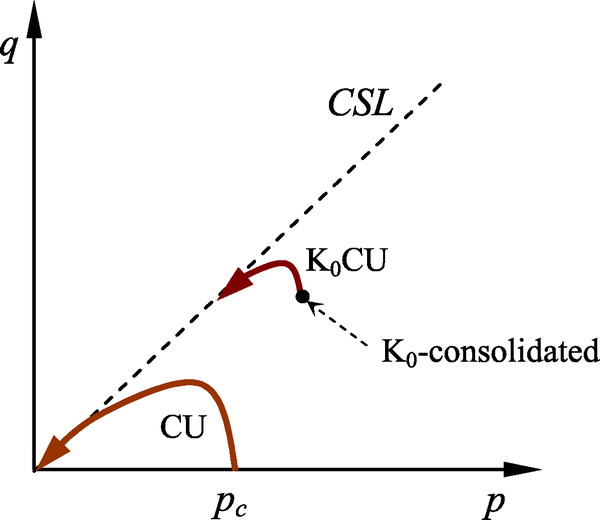
\includegraphics[width=.5\textwidth]{figures/figure2.jpg}
    \bicaption{Stress path analyzed (CU = consolidated undrained compression triaxial test; $K_{0}\mathrm{CU}=K_{0}$-consolidated undrained compression triaxial test; CSL = critical state line)}{应力路径分析(CU为固结不排水三轴试验; $K_{0}\mathrm{CU}$为$K_ {0}$固结不排水三轴试验; CSL为临界状态线)}
    \label{figure:2}
\end{figure}
    }
    \switchcolumn*

    in an infinitesimal deformation condition, according to the second-order work criterion, the stability of material requires

    \switchcolumn

    在无限小变形条件下,根据二阶功准则,材料的稳定性要求为

    \CrossColumnText{
        \begin{align}
            d^{2} w=d \widetilde{\sigma}^{\prime}: d \tilde{\varepsilon}>0, \quad \forall\|d \tilde{\varepsilon}\| \neq 0
            \label{equation:23}
        \end{align}
    }
    \switchcolumn*

    \noindent
    where $d^{2} w$ = second-order work; $d \widetilde{\sigma}^{\prime}$ = effective stress increment; and $d \tilde{\varepsilon}$ = corresponding strain increment.

    \switchcolumn

    \noindent
    式中,$d^{2} w$为二阶功,$d \widetilde{\sigma}^{\prime}$为有效应力增量,$d \tilde{\varepsilon}$为对应的应变增量。

    \switchcolumn*

    It could be inferred that, if there exists a loading path that results in the violation of \enautoref{equation:23}, the material becomes potentially unstable, so the condition of the potential instability is

    \switchcolumn

    可以推断出,如果存在导致违反\cnautoref{equation:23}的加载路径,则材料可能会变得不稳定,因此潜在的不稳定条件为

    \CrossColumnText{
        \begin{align}
            d^{2} w=d \widetilde{\sigma}^{\prime}: d \tilde{\varepsilon} \leq 0, \quad \exists\|d \tilde{\varepsilon}\| \neq 0
            \label{equation:24}
        \end{align}
    }

    \switchcolumn*

    \noindent
    After inserting \enautoref{equation:11} or \enautoref{equation:20}, one gets

    \switchcolumn

    \noindent
    将\cnautoref{equation:11}代入\cnautoref{equation:20},得到

    \CrossColumnText{
        \begin{align}
            d \tilde{\varepsilon}: \mathbf{D}^{e p}: d \tilde{\varepsilon} \leq 0, \quad \exists\|d \tilde{\varepsilon}\| \neq 0
            \label{equation:25}
        \end{align}
    }
    \switchcolumn*

    \noindent
    \enautoref{equation:25}implies the vanishing determinant value of the symmetric part

    \switchcolumn

    \noindent
    \cnautoref{equation:25}隐含着对称部分的行列式值

    \CrossColumnText{
        \begin{align}
            \operatorname{det}\left(\mathbf{D}_{\mathrm{sys}}^{e p}\right) \leq 0
            \label{equation:26}
        \end{align}
    }
    \switchcolumn*

    \noindent
    When under a triaxial condition, the criterion of \enautoref{equation:26} becomes

    \switchcolumn

    \noindent
    在三轴条件下,\cnautoref{equation:26}变为

    \CrossColumnText{
        \begin{align}
            \operatorname{det}\left[\left(\mathbf{D}_{p q}^{e p}\right)_{\mathrm{sys}}\right] \leq 0
            \label{equation:27}
        \end{align}
    }
    \switchcolumn*

    \enautoref{equation:24} also could be expressed by replacing the strain increment with stress rate

    \switchcolumn

    \cnautoref{equation:24}也可以通过用应力率代替应变增量来表示

    \CrossColumnText{
        \begin{align}
            d \widetilde{\boldsymbol{\sigma}}^{\prime}: \mathbf{C}^{e p}: d \widetilde{\boldsymbol{\sigma}}^{\prime} \leq 0, \quad \exists\left\|d \widetilde{\boldsymbol{\sigma}}^{\prime}\right\| \neq 0
        \end{align}
    }
    \switchcolumn*

    \noindent
    where $\mathbf{C}^{e p}$ = inversion of $\mathbf{D}^{e p}$. The determinant of the symmetric part of both tensors goes to zero simultaneously \citep{Prunier2009}, so the analysis based on both tensors would give the same results.

    \switchcolumn

    \noindent
    其中$\mathbf{C}^{e p}$为$\mathbf{D}^{e p}$的逆矩阵。 两个张量的对称部分的行列式同时变为零\citep{Prunier2009},因此基于两个张量的分析将得出相同的结果。

    \switchcolumn*

    It should be noted that Eqs. \ref{equation:26} and \ref{equation:27} are necessary but insufficient conditions of \enautoref{equation:25}. Once \enautoref{equation:26} is satisfied, the soil becomes potentially unstable and the stability depends on the stress increment. It could be inferred that the soil could stay stable as long as the stress increment is not along the unstable stress path, even if the soil is potentially unstable. Also, it should be noted that the negative value of the second-order work is necessary but insufficient for the static liquefaction \citep{Chu2001}, and the additional conditions are \citep{Lade1992}

    \switchcolumn

    应该注意的是,\cnautoref{equation:26}和\cnautoref{equation:27}是必要的,但\cnautoref{equation:25}的条件不足。 一旦\cnautoref{equation:26}满足,土体变得潜在不稳定,稳定性取决于应力增量。 可以推断,即使应力增加不沿着不稳定的应力路径,土体也可以保持稳定,即使土体可能是不稳定的。 另外,应该指出的是,二阶功的负值是必要的,但对于静态液化来说是不足的\citep{Chu2001},附加条件是\citep{Lade1992}。

    \CrossColumnText{
        \begin{align}
            \begin{array}{l}
            \frac{\partial F}{\partial \sigma_{i j}} \cdot \delta_{i j}<0 \\
            \frac{\partial Q}{\partial \sigma_{i j}} \cdot \delta_{i j}>0
            \end{array}
            \label{equation:29}
        \end{align}
    }
    \switchcolumn*

    \noindent
    By substituting Eqs. \ref{equation:3} and \ref{equation:8} into \enautoref{equation:29}, the first inequality is satisfied, and the second inequality requires $M_d-M>0$. It can be concluded that the tendency of volumetric compression of the soil under undrained conditions combined with the violation of second-order work yield the complete condition for static liquefaction to occur.

    \switchcolumn

    \noindent
    通过将\cnautoref{equation:3}和\cnautoref{equation:8}代入\cnautoref{equation:29},第一个不等式得到满足,第二个不等式要求$M_d-M>0$。 可以得出结论,在不排水的条件下土体的体积压缩趋势加上违反二阶功的情况为静态液化发生提供了完整条件。

\end{ParaColumn}
\begin{ParaColumn}[\bisection*{Experimental Predictions}{实验预测}]
    
    To assess the proposed model and the criteria of static liquefaction, experimental results (e.g., undrained triaxial test) are required for validation. There are two kinds of loading modes for undrained triaxial tests: (1) load-controlled loading mode, and (2) deformation-controlled loading mode. In load-controlled triaxial tests, instability occurs along with the sudden increase of strain rate, whereas in deformation-controlled tests, prefailure strain softening takes places under the same other conditions \citep{Chu2001}. Although both phenomena are different, the mechanism that governs the onset of instability is the same and could be predicted by the same criteria \citep{Chu2001, Chu2009}. Because this study focused on the onset of static liquefaction instability and the soil behavior at postpeak stage is beyond the study’s scope, only the deformation-controlled triaxial tests were analyzed.

    \switchcolumn

    为了评估建议的模型和静态液化标准,需要使用实验结果(例如不排水的三轴试验)进行验证。 不排水的三轴试验有两种加载方式:(1)荷载控制的加载方式和(2)变形控制的加载方式。 在载荷控制的三轴试验中,不稳定性随应变速率的突然增加而发生,而在变形控制的试验中,失效前的应变软化在相同的其他条件下发生\citep{Chu2001}。 尽管两种现象都不同,但控制不稳定性发作的机制是相同的,并且可以用相同的标准进行预测\citep{Chu2001, Chu2009}。 由于本研究的重点是静态液化不稳定性的发生,并且峰后阶段的土体行为超出了研究范围,因此仅分析了变形控制的三轴试验。

    \switchcolumn*[\bisubsection*{Isotropically Consolidated Undrained Triaxial Tests}{各向同性固结不排水三轴试验}]

    The proposed constitutive model and the instability criteria were used to predict the results of the isotropically consolidated undrained triaxial tests of \citet{Doanh1997}. The specimen, which was 70 mm in diameter and 70 mm in height, was made of Hostun RF sand with minimum void ratio $e_{\min} = 0.648$ and maximum void ratio $e_{\max} = 1.041$. The void ratios of the specimen after isotropical consolidation were 0.883, 0.875, and 0.854. The initial effective consolidation pressures of the tests were 100, 200, and 300 kPa.

    \switchcolumn

    提出的本构模型和不稳定性标准被用来预测\citet{Doanh1997}的各向同性固结不排水三轴试验的结果。 直径为70毫米,高度为70毫米的样品是由Hostun RF砂制成的,其最小孔隙比$e_{\min} = 0.648$,最大孔隙比$e_{\max} = 1.041$。 各向同性固结后,试样的孔隙比分别为0.883、0.875和0.854。 试验的初始有效固结压力为100、200和300 kPa。

    \CrossColumnText{
        \begin{figure}[htb]
    \centering
    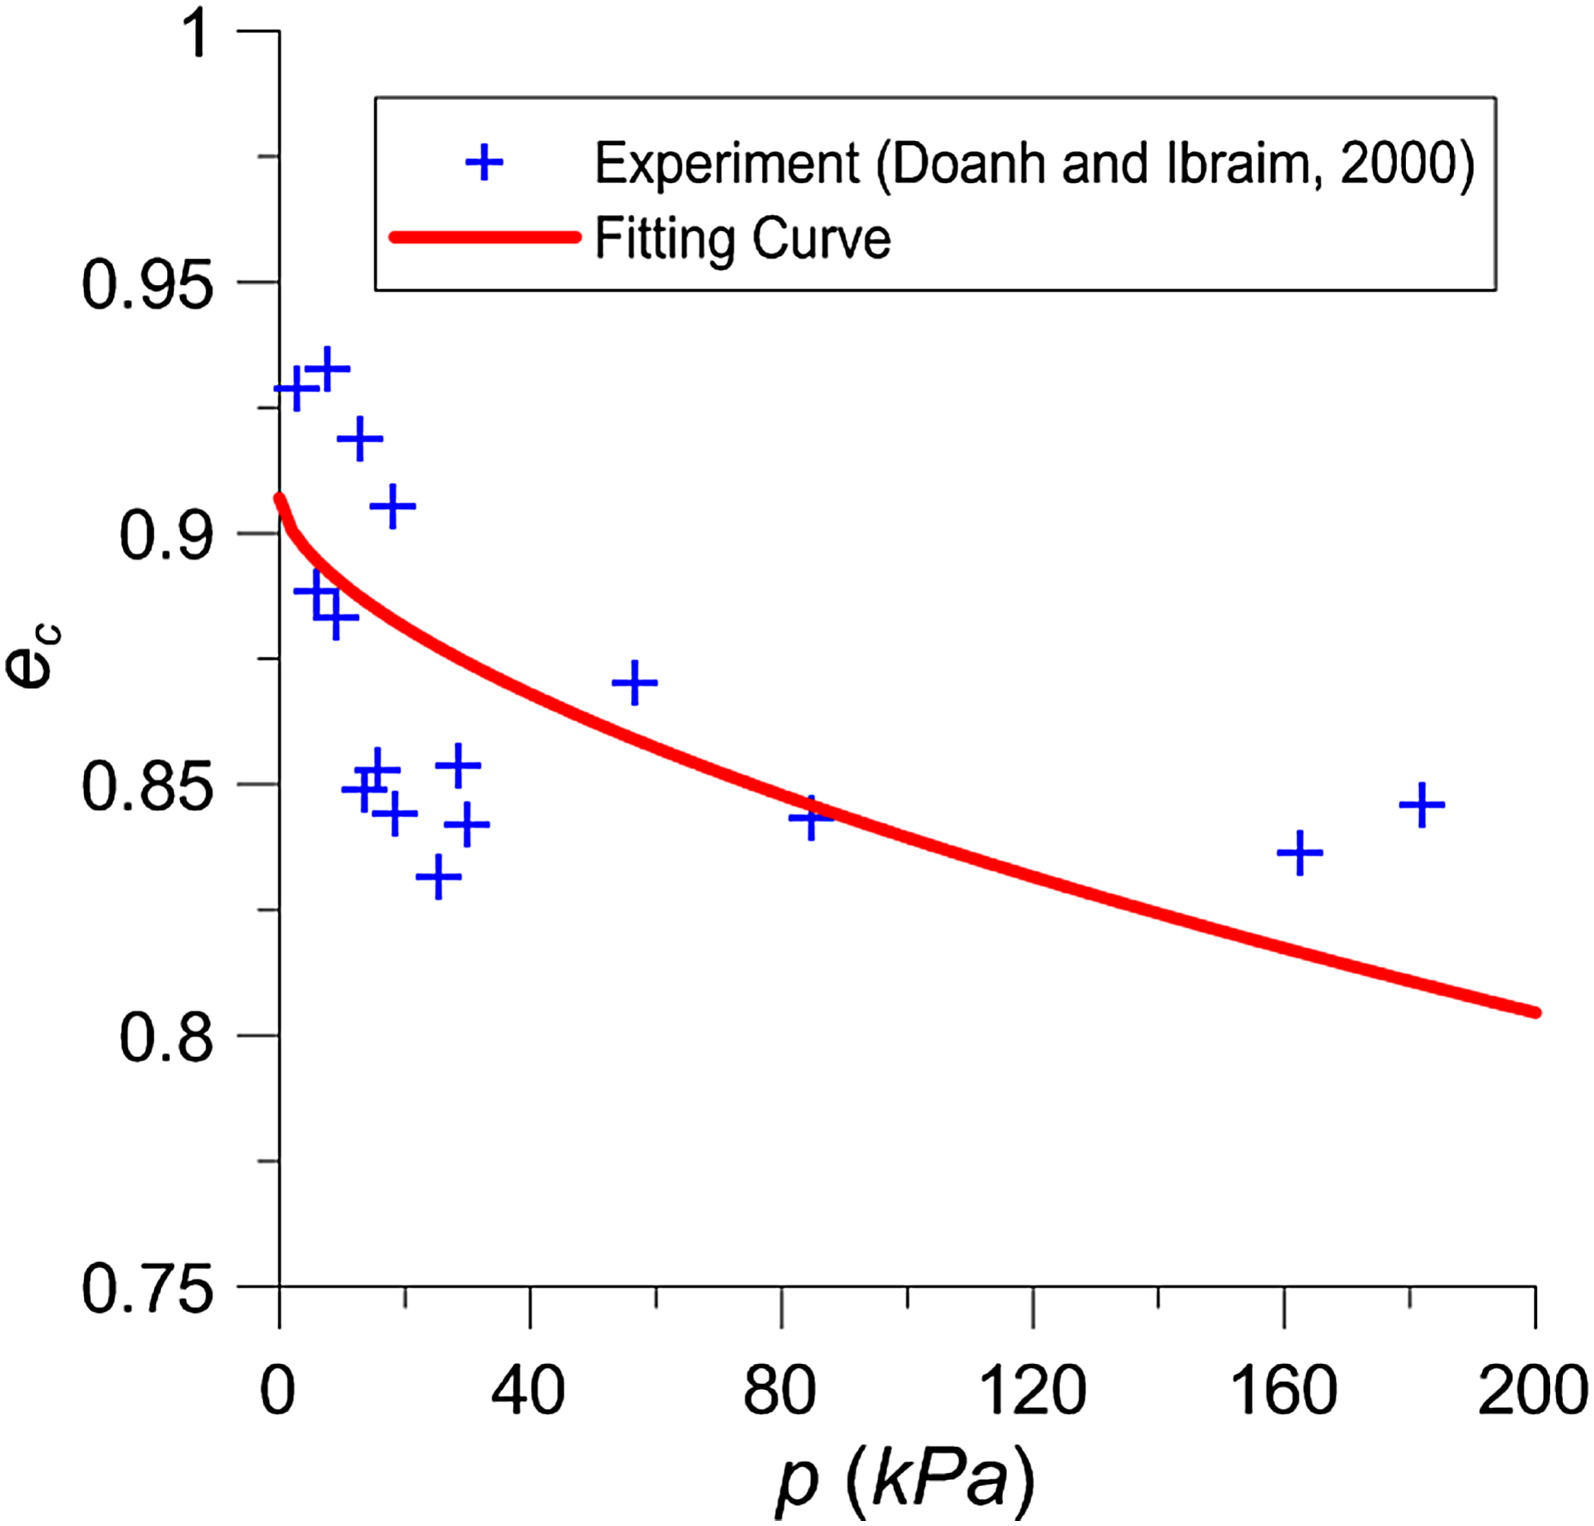
\includegraphics[width=.5\textwidth]{figures/figure3.jpg}
    \bicaption{The  $e_c-p$  curve at critical state (experimental data from \citet{Doanh2000})}{临界状态下的$e_c-p$曲线(来自\citet{Doanh2000}的实验数据)}
    \label{figure:3}
\end{figure}
    }
    \switchcolumn*

    The elastic parameter $G_{0}$ is a regression constant and could be determined by fitting a series of independent small-strain test data (e.g., from bender element tests) using \enautoref{equation:14}; Poisson's ratio $\nu$ could be determined by \enautoref{equation:14} when the bulk modulus was known. The parameter $M_{c s}$ and parameters $\lambda_{c}, e_{c 0},$ and $\xi$ were determined by fitting the experimental data of the stress ratio and $e-p$ data at the critical state. The obtained $e_{c}-p$ curve of Hostun $\mathrm{RF}$ sand (Doanh and Ibraim 2000 ) is shown in \enautoref{figure:3} The $n_{b}$ could be determined by \enautoref{equation:5} from the measured data of $\psi$ and $M$ at the phase-transformation state, $n_{d}$ could be determined by \enautoref{equation:7} from the measured data of $\psi$ and $M$ at the drained peak stress state, and $d_{0}$ could be determined by the $\varepsilon_{v}-\varepsilon_{q}$ curve from the drained triaixal test. A fitting parameter $A$ could be obtained by fitting the stress-strain relationships.

    \switchcolumn

    弹性参数$G_{0}$是一个回归常数,可以通过使用等式拟合一系列独立的小应变试验数据(例如,来自弯曲元试验)使用\cnautoref{equation:14}来确定。当体积模量已知时泊松比$\nu$可由\cnautoref{equation:14}确定。参数$M_{cs}$和参数$\lambda_{c}$,$e_{c0}$和$\xi$是通过在临界状态下拟合应力比和$e-p$的实验数据来确定的。获得的Hostu n$\mathrm{RF}$砂土的$e_{c}-p$曲线\citep{Doanh2000}如\cnautoref{figure:3}所示。$n_{b}$可以由\cnautoref{equation:5}确定。从相变状态下的$\psi$和$M$的测量数据中,可以用\cnautoref{equation:7}从在排水状态下的$\psi$和$M$的测量数据确定$n_{d}$峰值应力状态,$d_{0}$可以通过排水三轴试验的$\varepsilon_{v}-\varepsilon_{q}$曲线确定。通过拟合应力应变关系可以获得拟合参数$A$。

    \switchcolumn*

    After all the material parameters were calibrated (listed in \cnautoref{table:1}), the behavior of the specimen was predicted by deformation-controlled loading. As shown in \enautoref{figure:4}, the predicted effective stress path under undrained loading process compared very well with the experiments. The predicted effective stress-strain relationship and pore-water pressure are shown in \enautoref{figure:5}; the deviatoric shear stress rapidly increased to the peak, and then decreased along with the continuous increase in pore-water pressure. During the loading process, the determinant of the symmetric elastoplastic modulus tensor and second-order work were calculated. As shown in \enautoref{figure:6}, both values vanished simultaneously at the peak of the deviatoric stress, which indicates that the static liquefaction started when the soil entered into the potentially unstable state. The evolution of the hardening modulus Hp is shown in \enautoref{figure:7}; the static liquefaction occurred at the hardening stage of the soil. The difference between these results and those of \citet{Andrade2009}, in which static liquefaction occurred at the softening regime of the soil, is due to the adoption of a different kind of constitutive model.

    \switchcolumn

    校准所有材料参数(在\cnautoref{table:1}中列出)后,通过变形控制载荷预测样品的行为。如\cnautoref{figure:4}所示,在不排水的加载过程中预测的有效应力路径与实验结果非常吻合。预测的有效应力应变关系和孔隙水压力如\cnautoref{figure:5}所示。偏剪应力迅速增加到峰值,然后随着孔隙水压力的不断增加而减小。在加载过程中,计算了对称弹塑性模量张量的决定因素和二阶功。如\cnautoref{figure:6}所示,这两个值在偏应力峰值时同时消失,这表明当土体进入潜在不稳定状态时,静态液化开始。硬化模量Hp的变化如\cnautoref{figure:7}所示。静态液化发生在土体的硬化阶段。这些结果与\citet{Andrade2009}的结果之所以不同,是由于采用了另一种本构模型,在土体的软化状态下发生了静态液化。

    \CrossColumnText{
        \begin{table}[htbp]
    \centering
    \bicaption{Material Parameters Used in the Simulation [Experimental Data from \citet{Doanh1997} and \citet{Chu2008}]}{模拟中使用的材料参数[实验数据来自\citet{Doanh1997}以及\citet{Chu2008}]}
    \label{table:1}
    \begin{tabularx}{\textwidth}{lll}
        \toprule
        Material parameters & Istropically consolidated undrained triaxial tests & $K_0$-consolidated undrained triaxial tests \\
        \midrule
        $G_0$ & 125 & 30 \\
        $\nu$ & 0.15 & 0.05 \\
        $M_{cs}$ & 1.0 & 1.35\\
        $\lambda_c$ & 0.078 & 0.098 \\
        $e_{c0}$ & 0.907 & 0.972 \\
        $\xi$ & 0.6 & 0.4 \\
        $n_b$ & 1.1 & 1.1 \\
        $n_d$ & 3.5 & 3.5 \\
        $d_0$ & 0.88 & 0.88 \\
        $A$ & 0.001 & 0.003 \\
        \bottomrule
    \end{tabularx}
\end{table}
        \begin{figure}[p]
    \centering
    \begin{minipage}[b]{.48\textwidth}
        \begin{figure}[H]
            \centering
            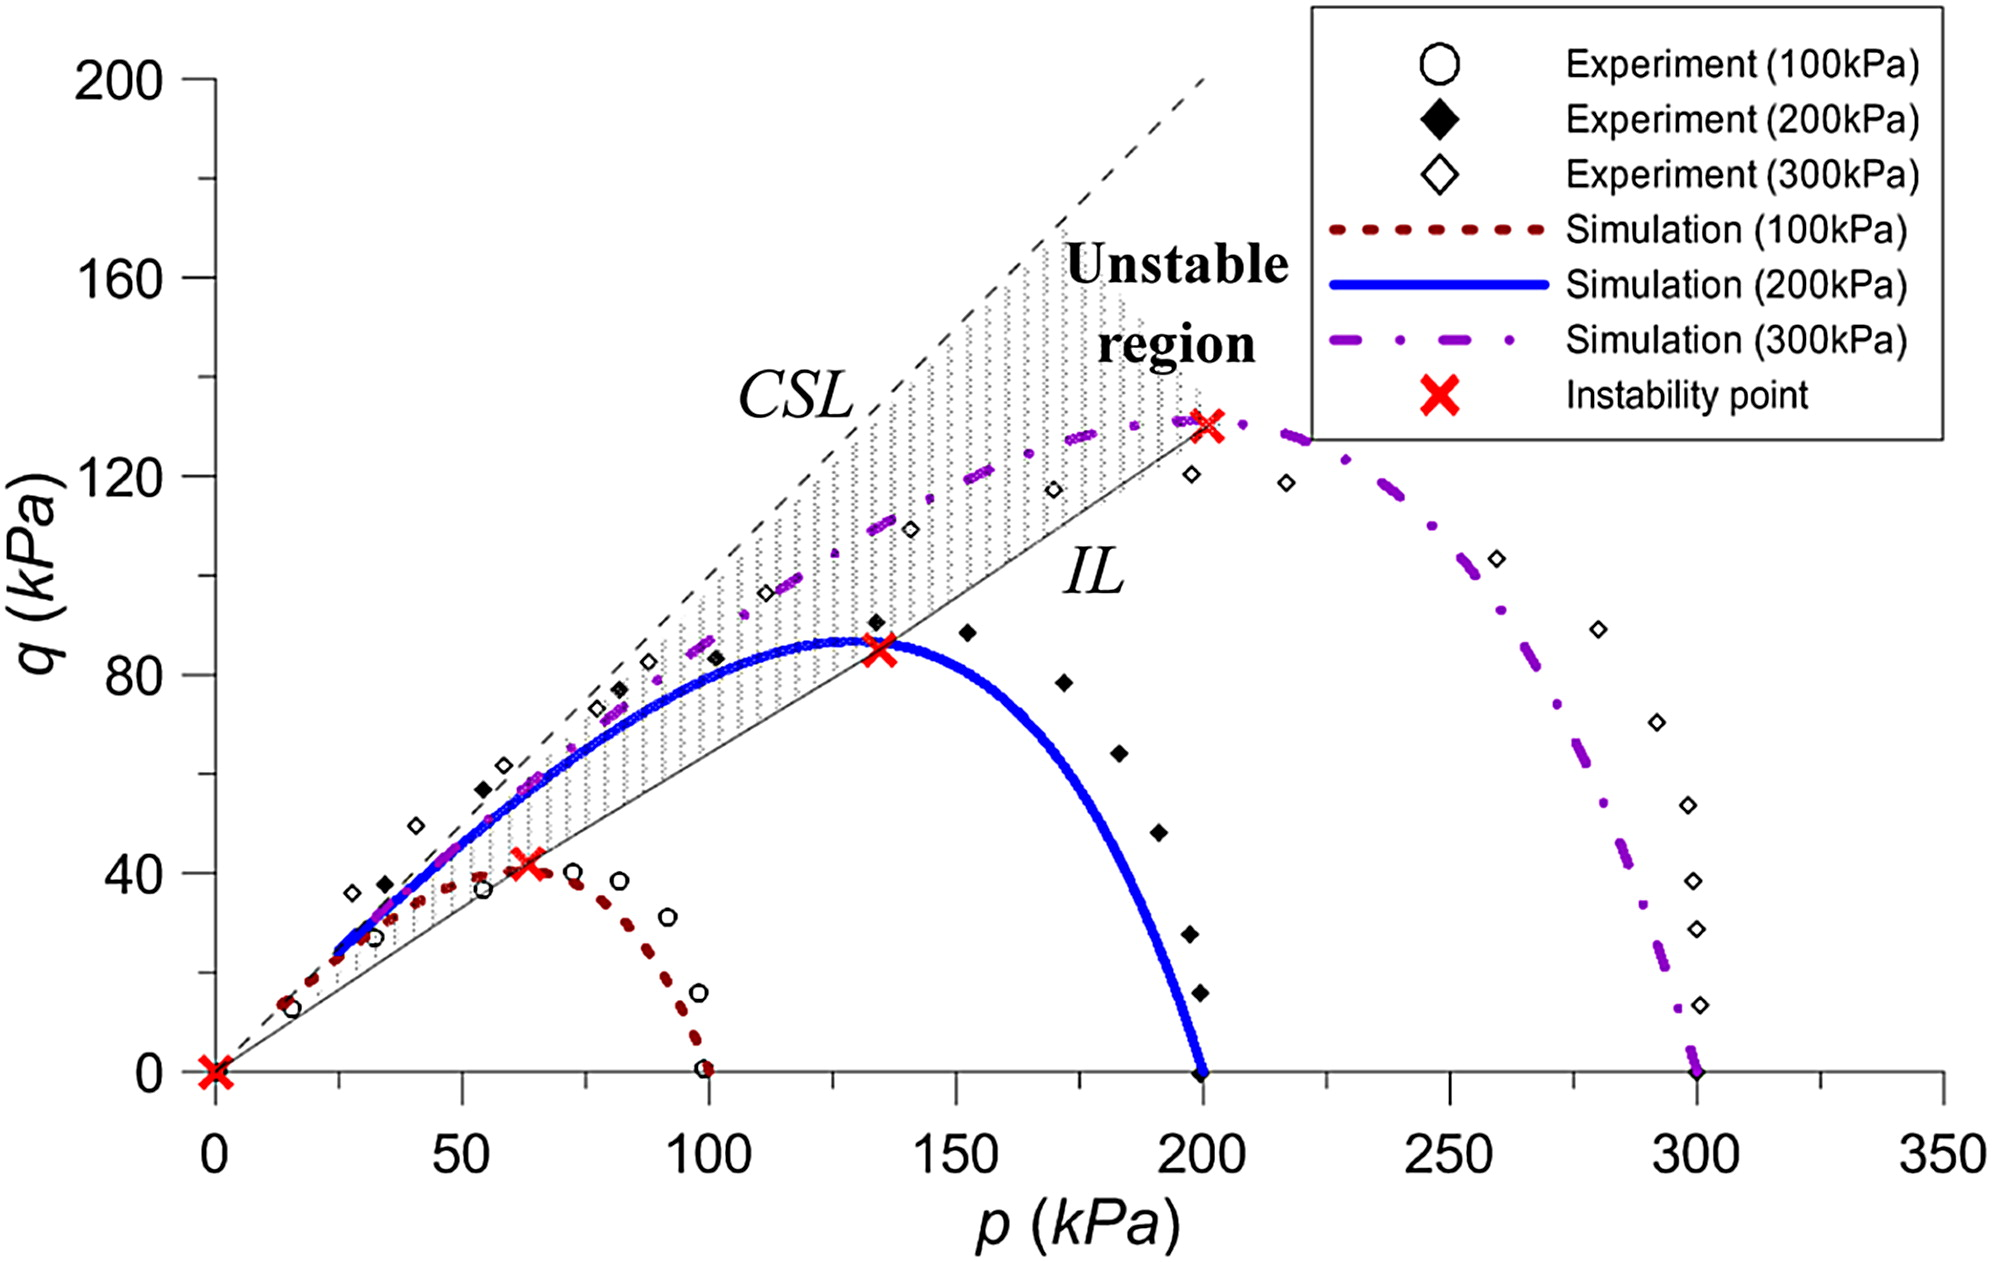
\includegraphics[width=.75\textwidth]{figures/figure4.jpg}
            \bicaption{Stress path of isotropically consolidated undrained triaxial test (experimental data from \citet{Doanh1997})}{各向同性固结不排水三轴试验的应力路径(实验数据来自\citet{Doanh1997})}
            \label{figure:4}
        \end{figure}
        \begin{figure}[H]
            \centering
            \addtocounter{figure}{1}
            \subfigure[determinant of the symmetric part of the elastoplastic modulus tensor 弹塑性模量张量的对称部分的行列式的演变]{
                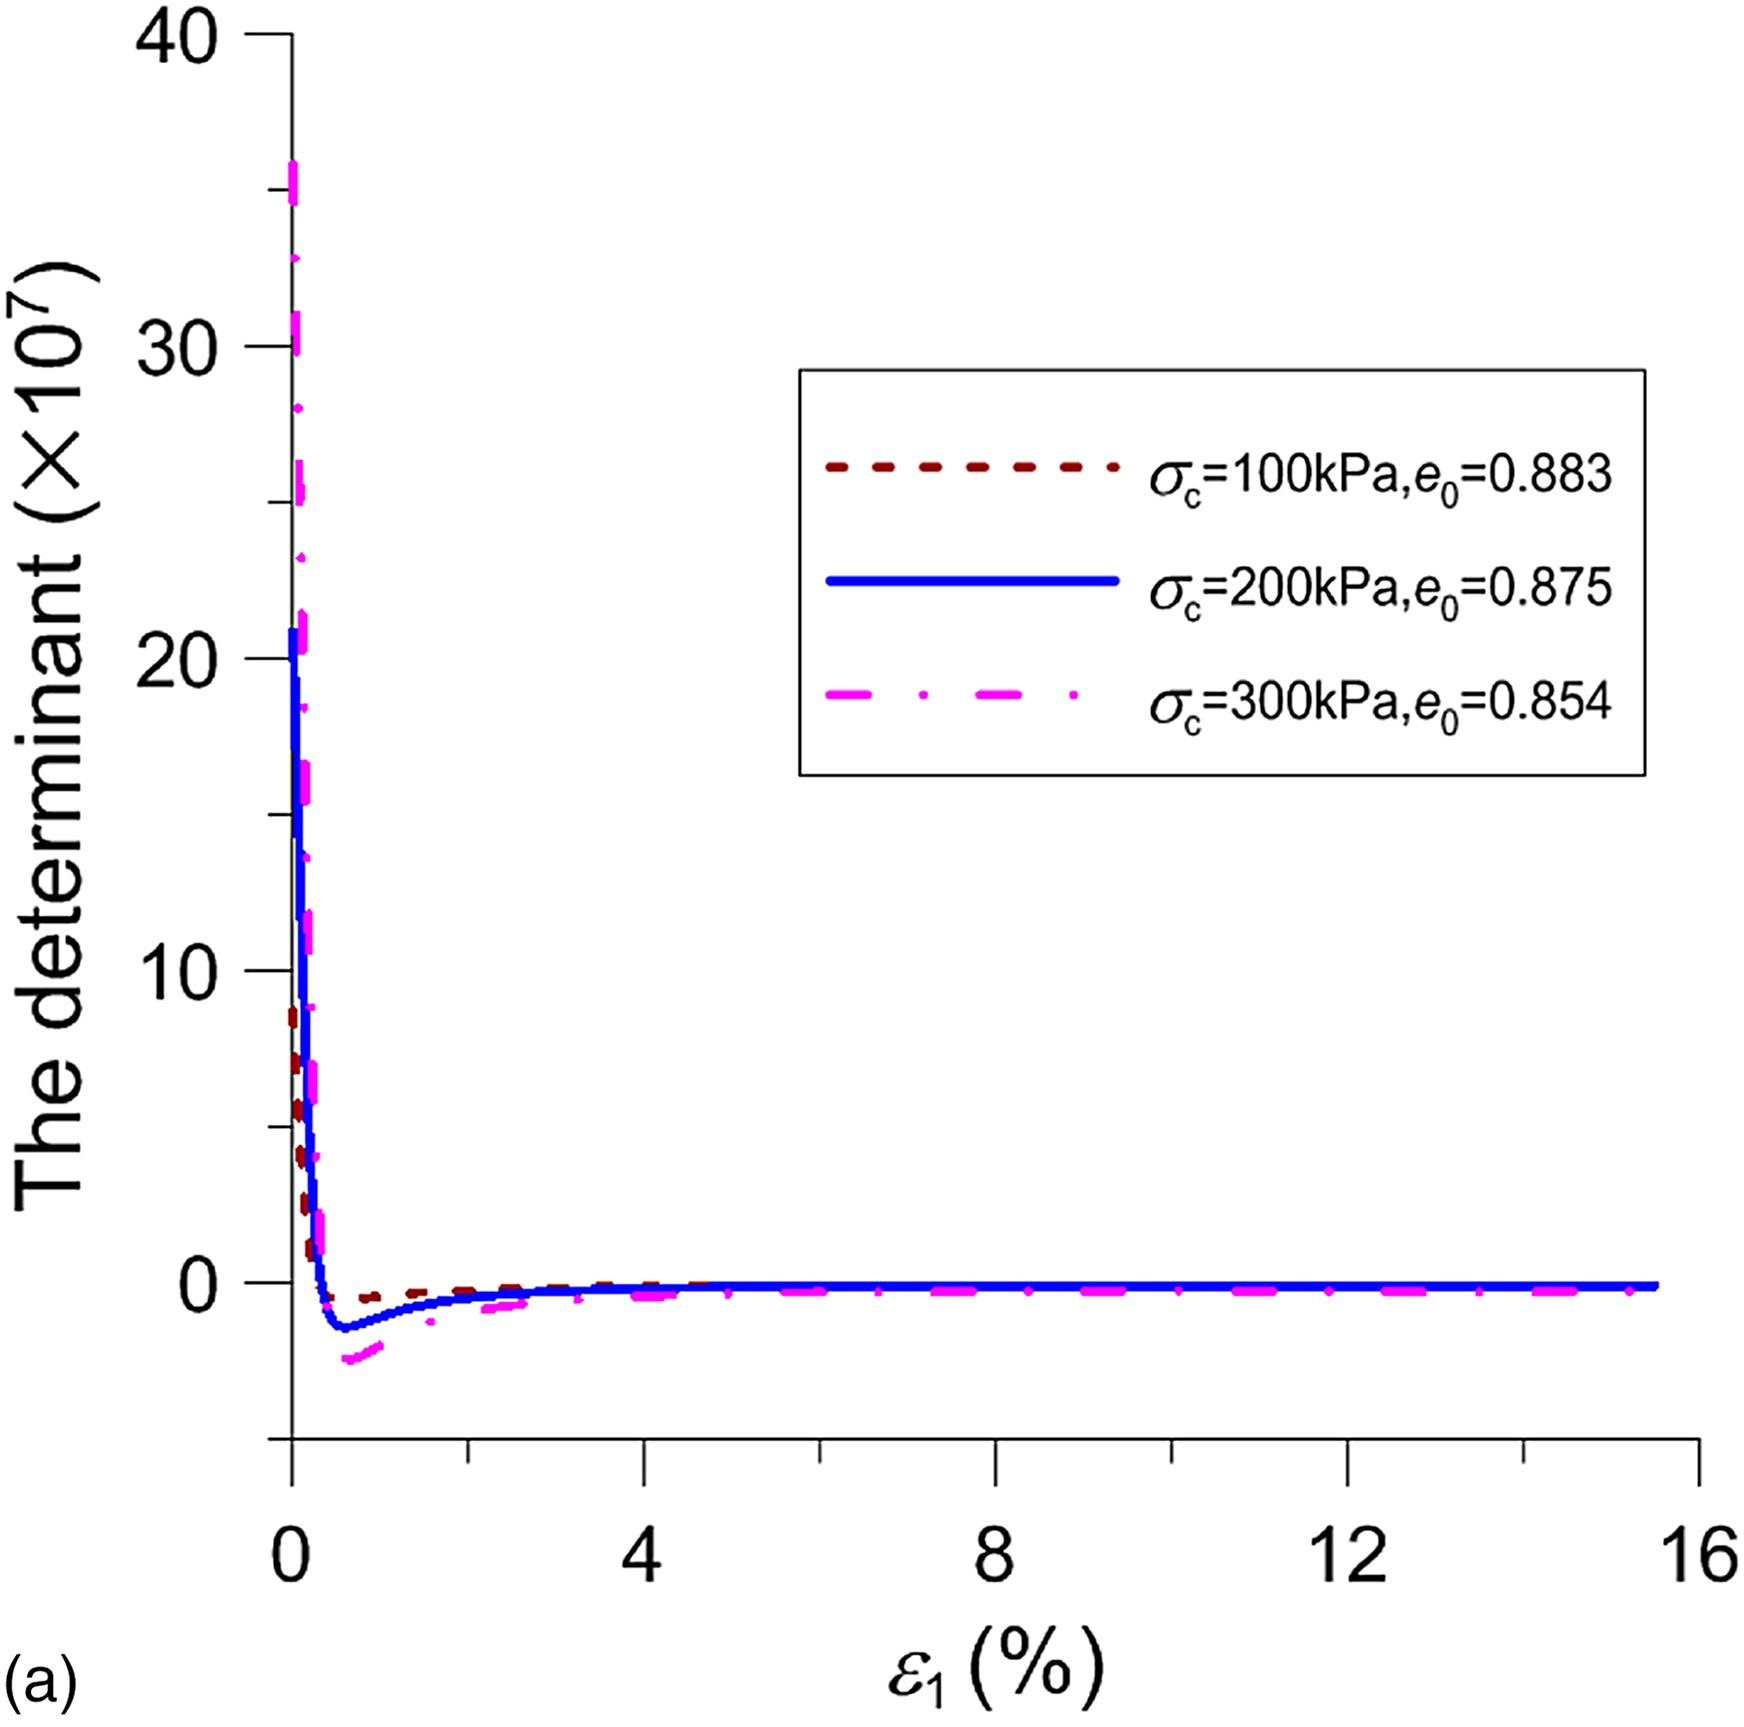
\includegraphics[width=.75\textwidth]{figures/figure6a.jpg}
                \label{figure:6a}
            }
            \subfigure[evolution of second-order work 二阶功]{
                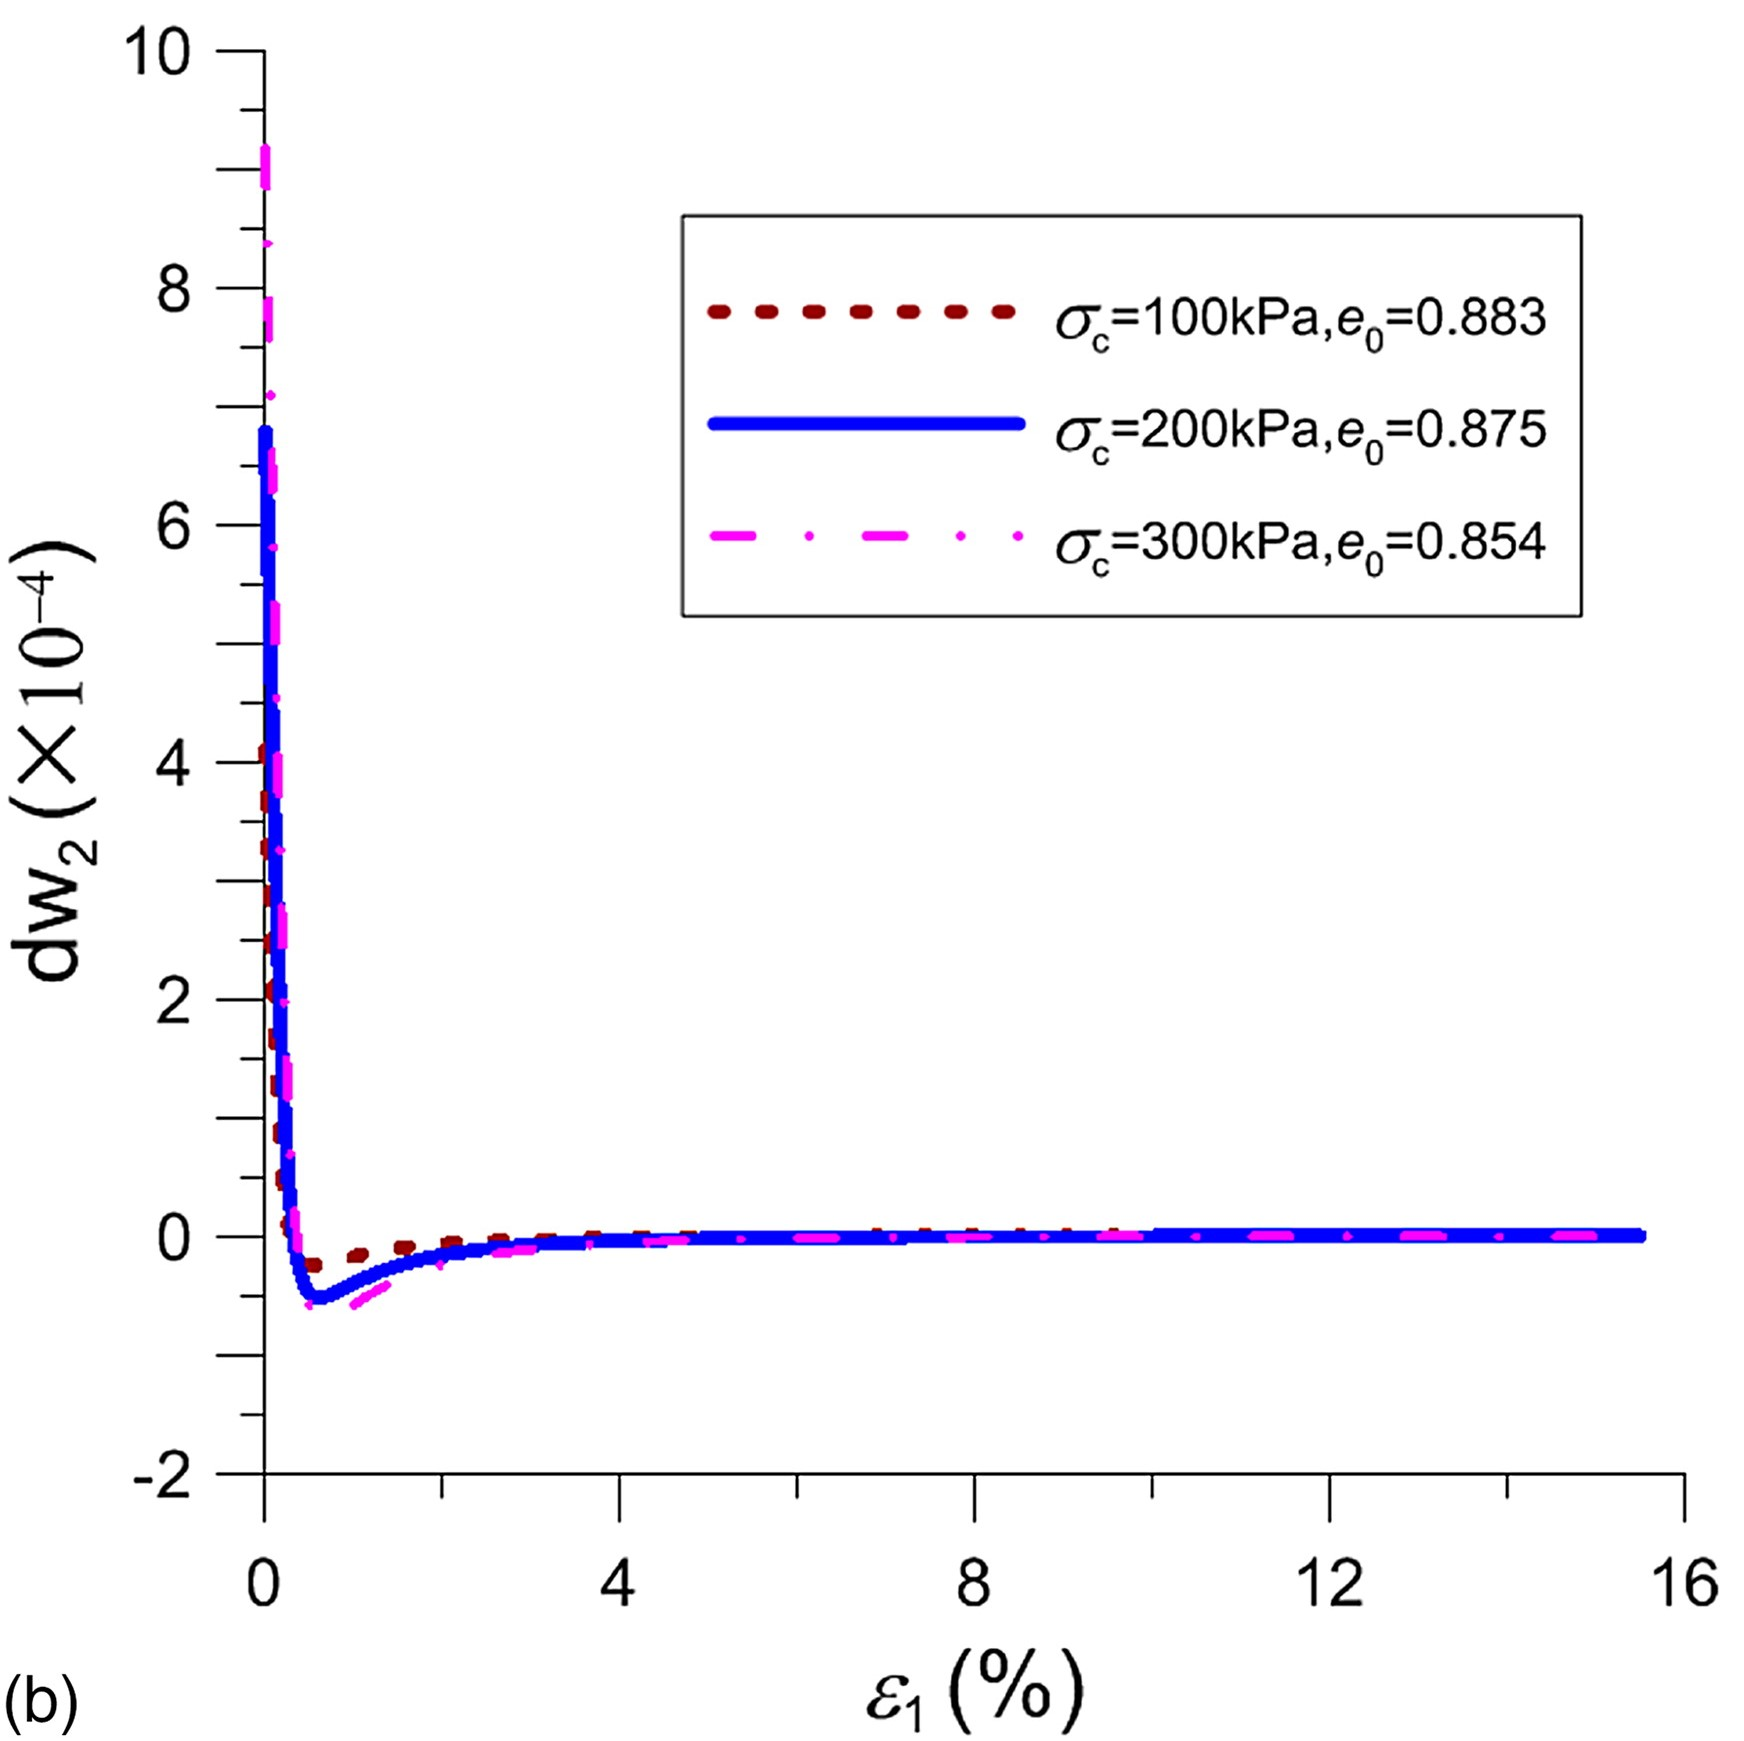
\includegraphics[width=.75\textwidth]{figures/figure6b.jpg}
                \label{figure:6b}
            }
            \bicaption{Evolution of determinant of the symmetric part of the elastoplastic modulus tensor and second-order work}{弹塑性模量张量的对称部分的行列式的和二阶功的演变}
            \label{figure:6}
        \end{figure}
    \end{minipage}
    \hspace{0.02\textwidth}
    \begin{minipage}[b]{.48\textwidth}
        \begin{figure}[H]
            \centering
            \addtocounter{figure}{-2}
            \subfigure[deviatoric stress, major principal strain 偏应力,主应变]{
                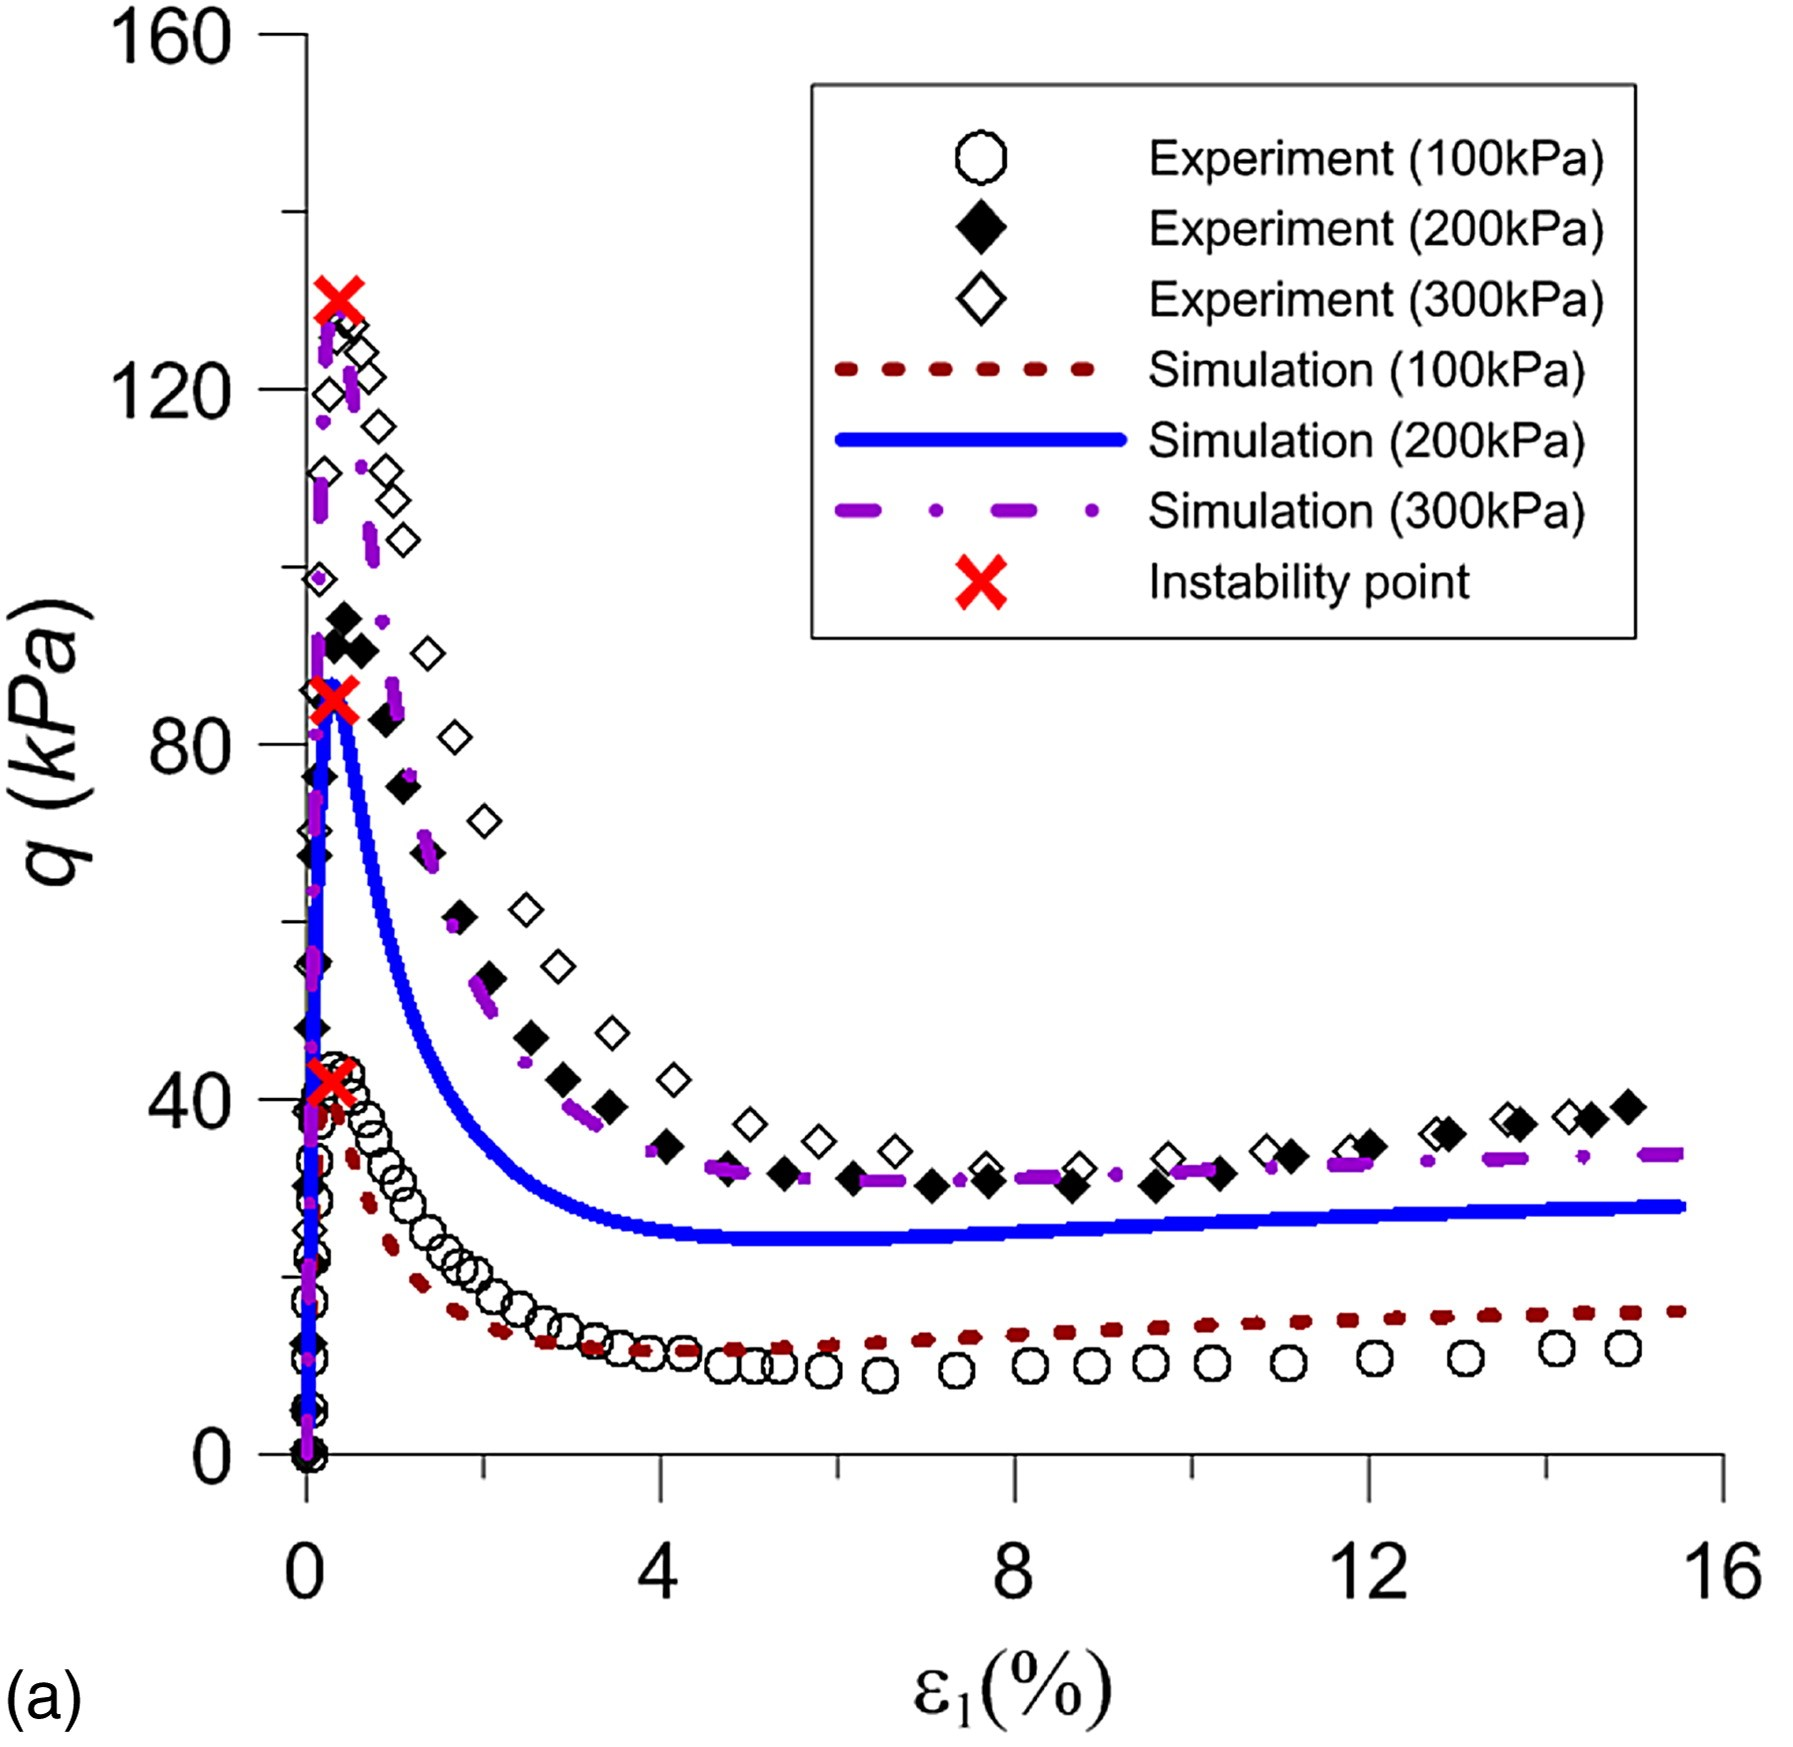
\includegraphics[width=.75\textwidth]{figures/figure5a.jpg}
                \label{figure:5a}
            }
            \subfigure[normalized pore pressure, major principal strain 归一化孔隙水压力,主应变]{
                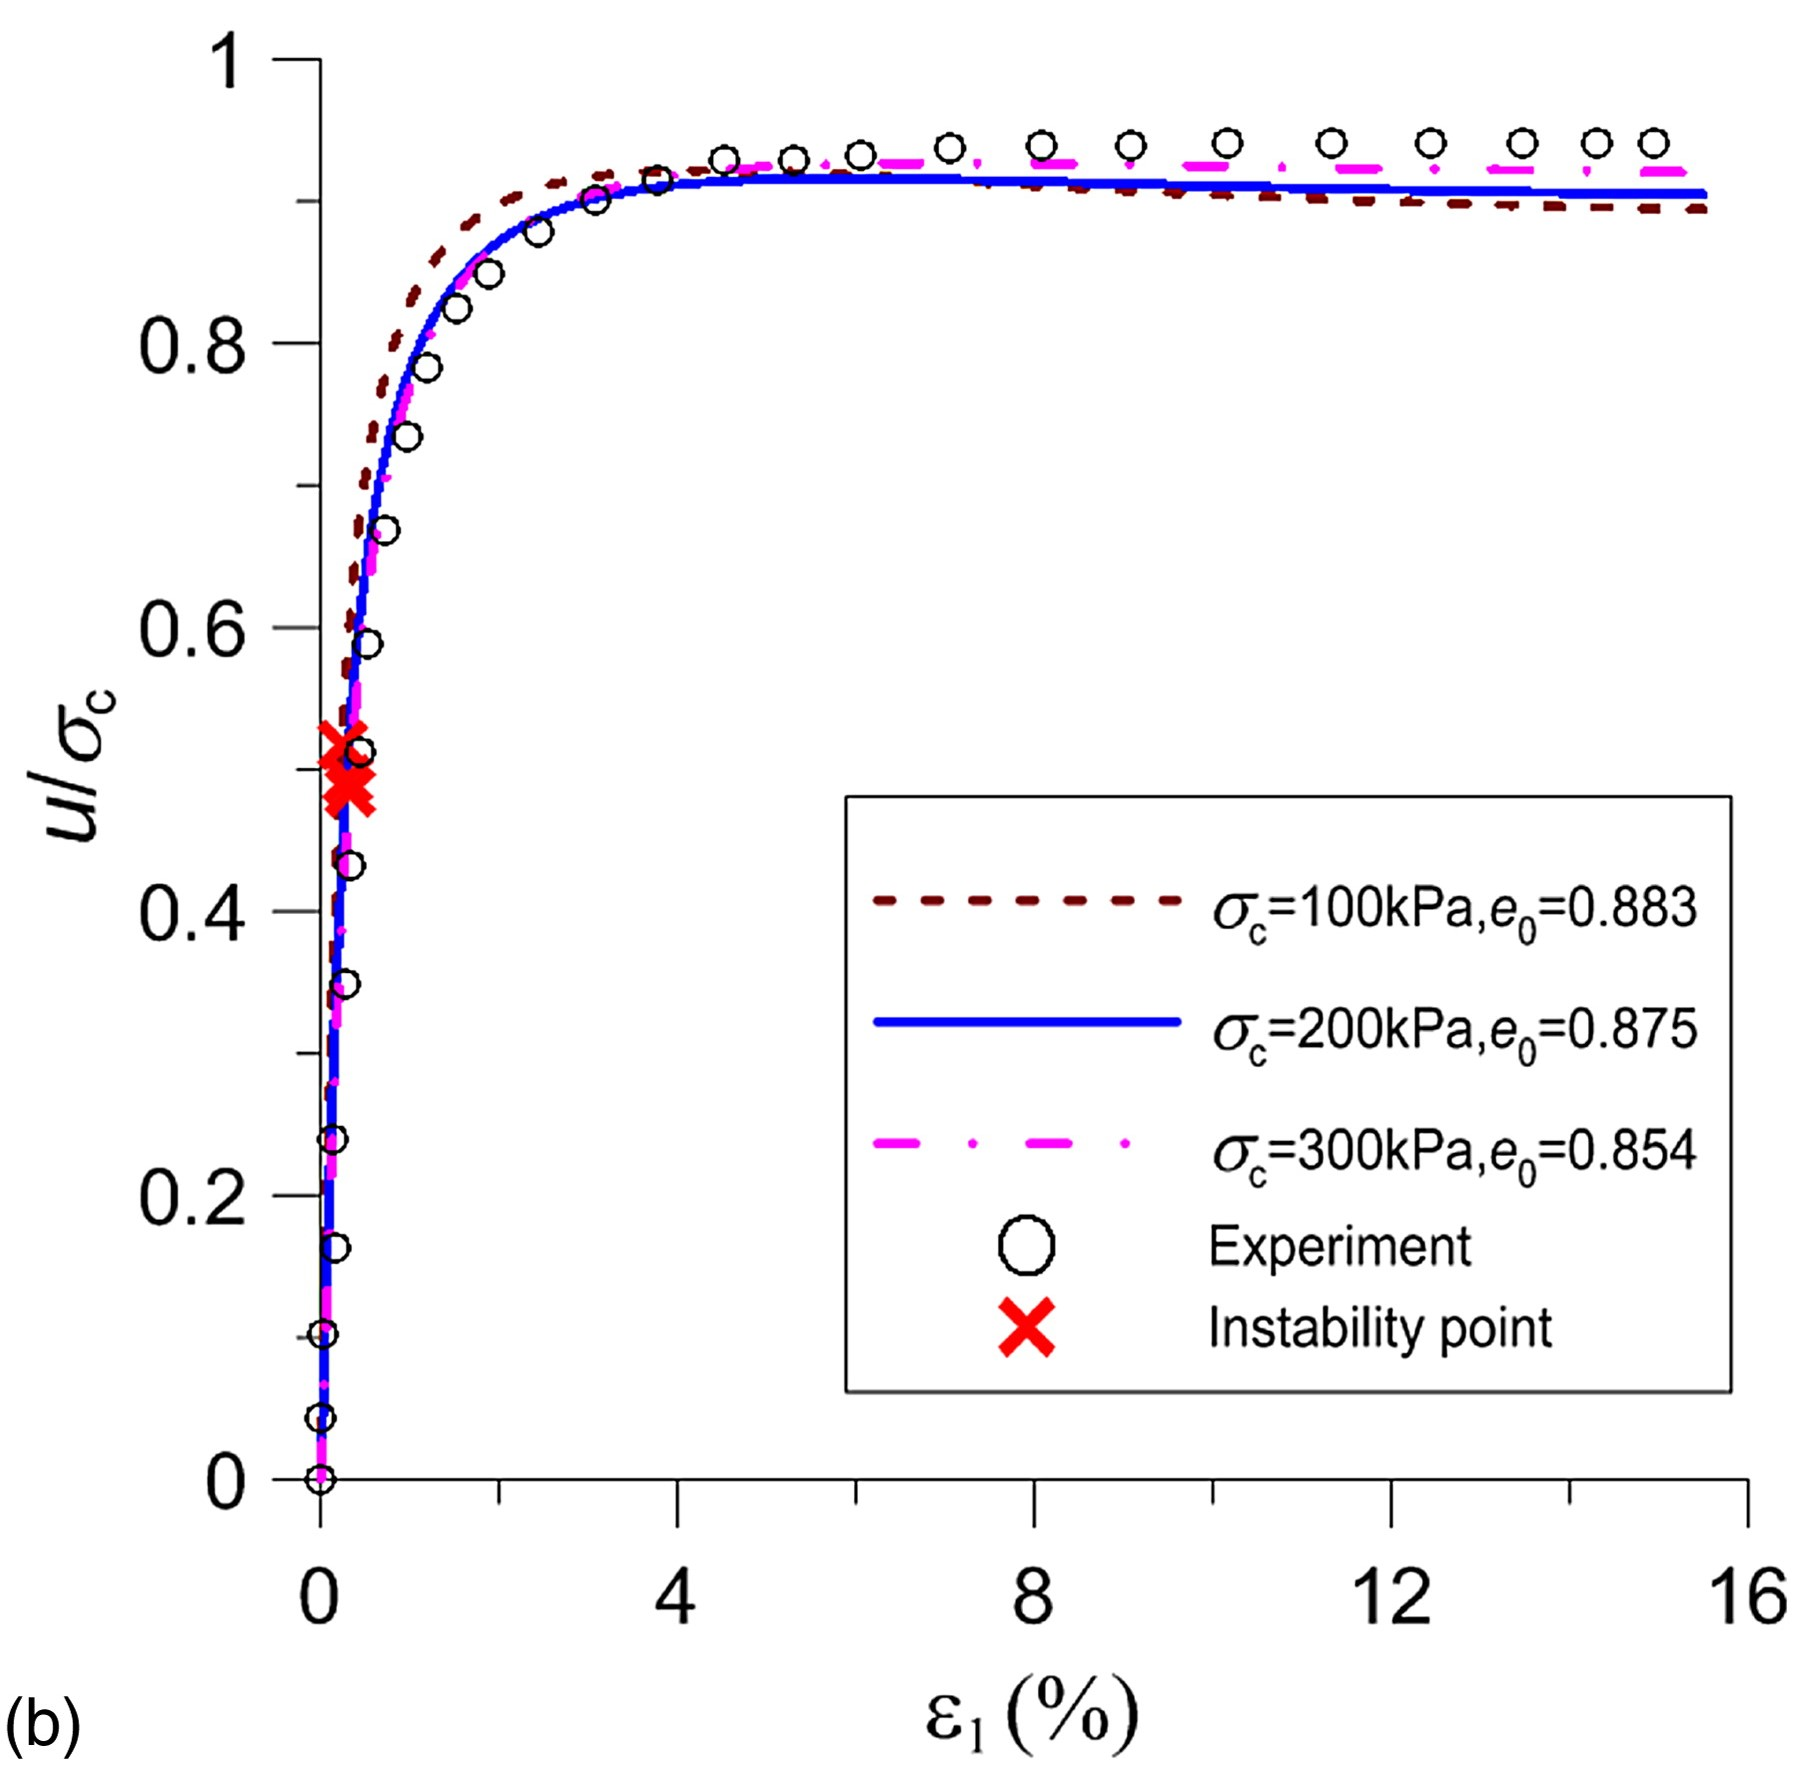
\includegraphics[width=.75\textwidth]{figures/figure5b.jpg}
                \label{figure:5b}
            }
            \bicaption{Model prediction (experimental data from \citealt{Doanh1997})}{模型预测(实验数据来自\citealt{Doanh1997})}
            \label{figure:5}
        \end{figure}
        \begin{figure}[H]
            \centering
            \addtocounter{figure}{1}
            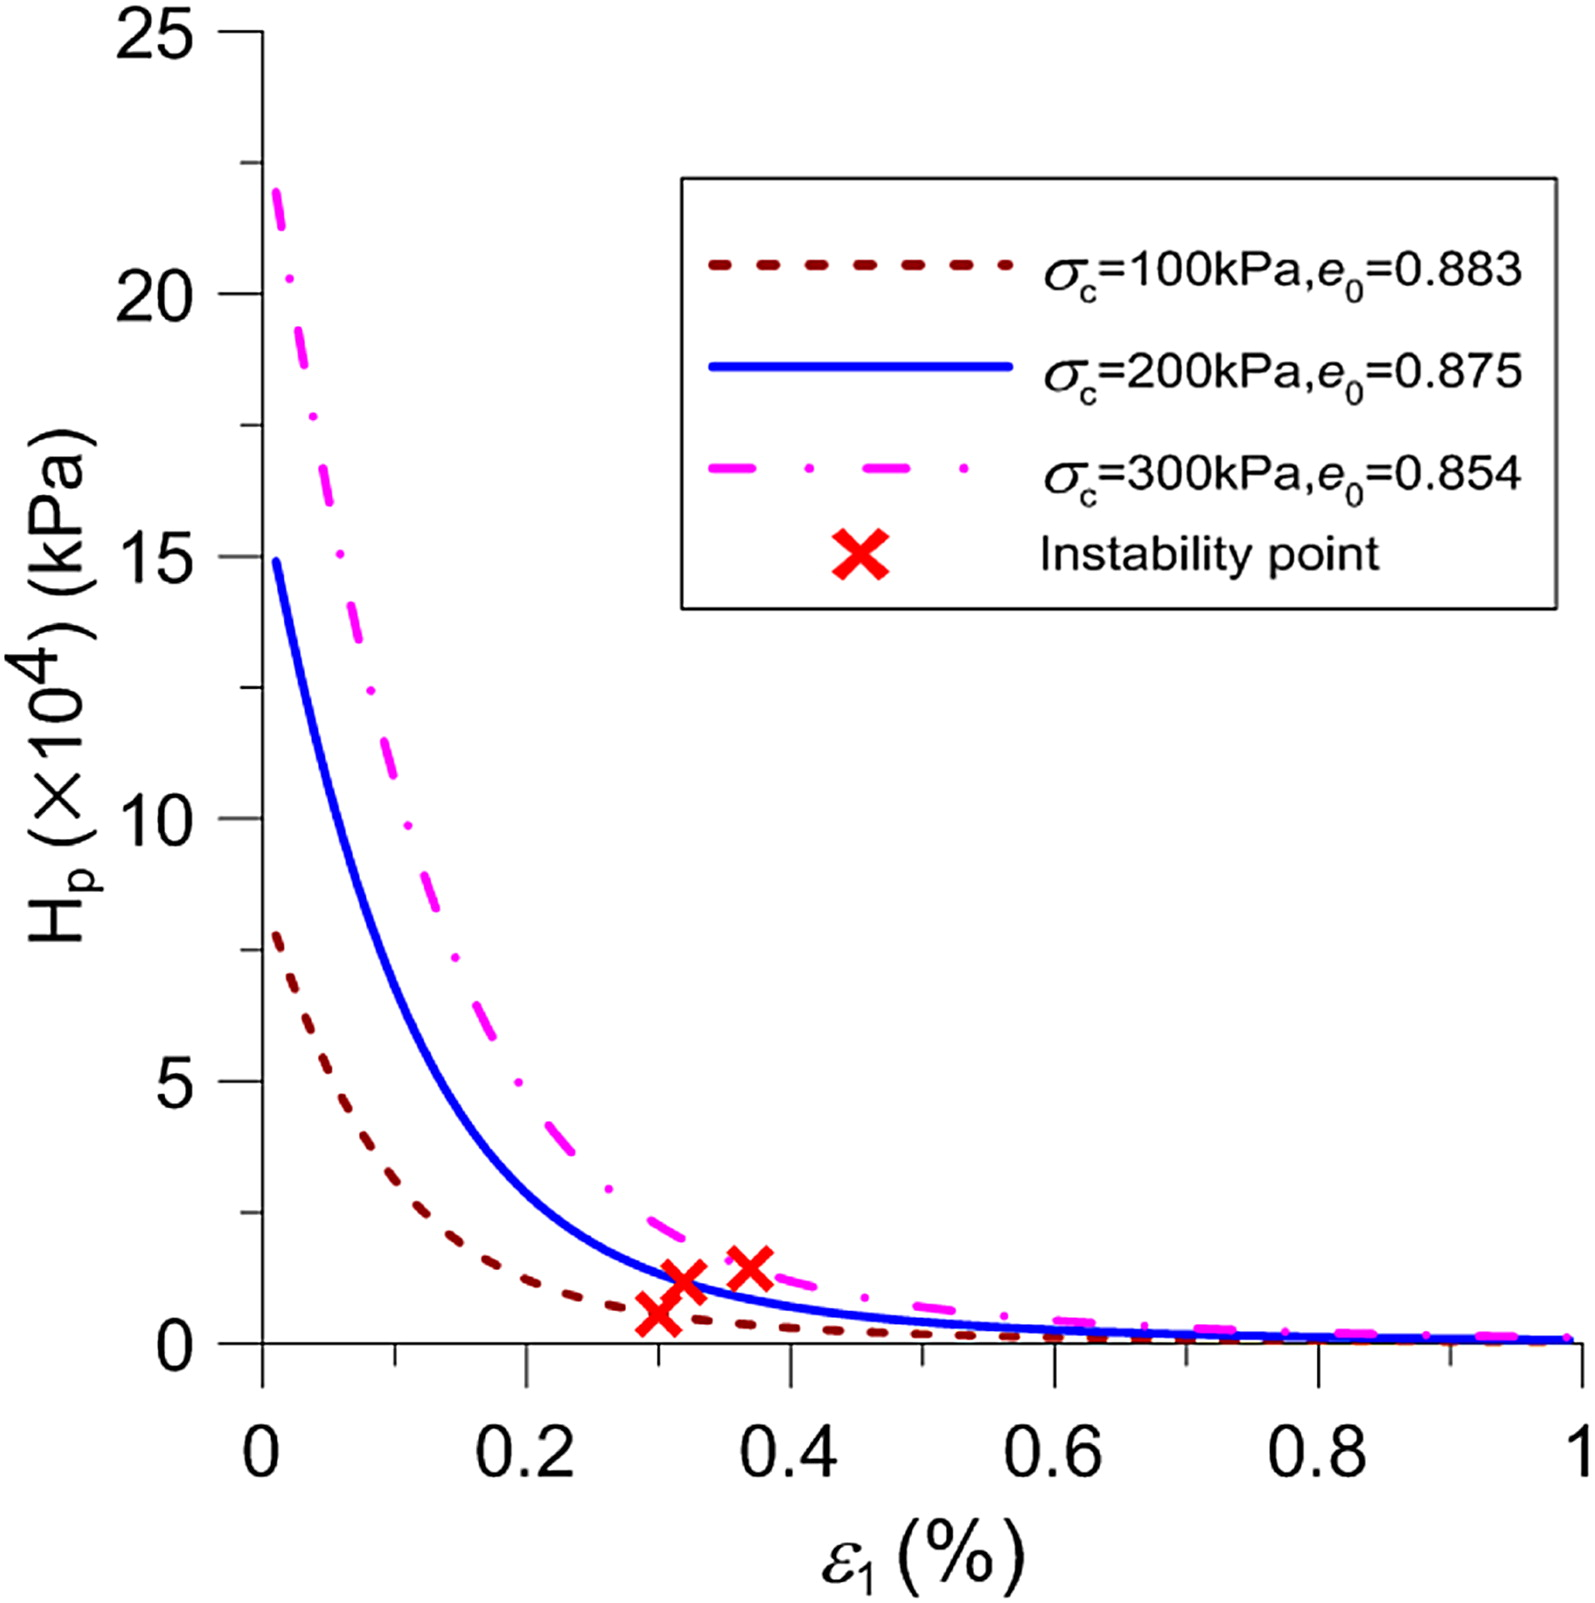
\includegraphics[width=.75\textwidth]{figures/figure7.jpg}
            \bicaption{Evolution of hardening modulus}{硬化模量的演变}
            \label{figure:7}
        \end{figure}
    \end{minipage}
\end{figure}
        \begin{figure}[p]
    \centering
    \begin{minipage}[b]{.48\textwidth}
        \begin{figure}[H]
            \centering
            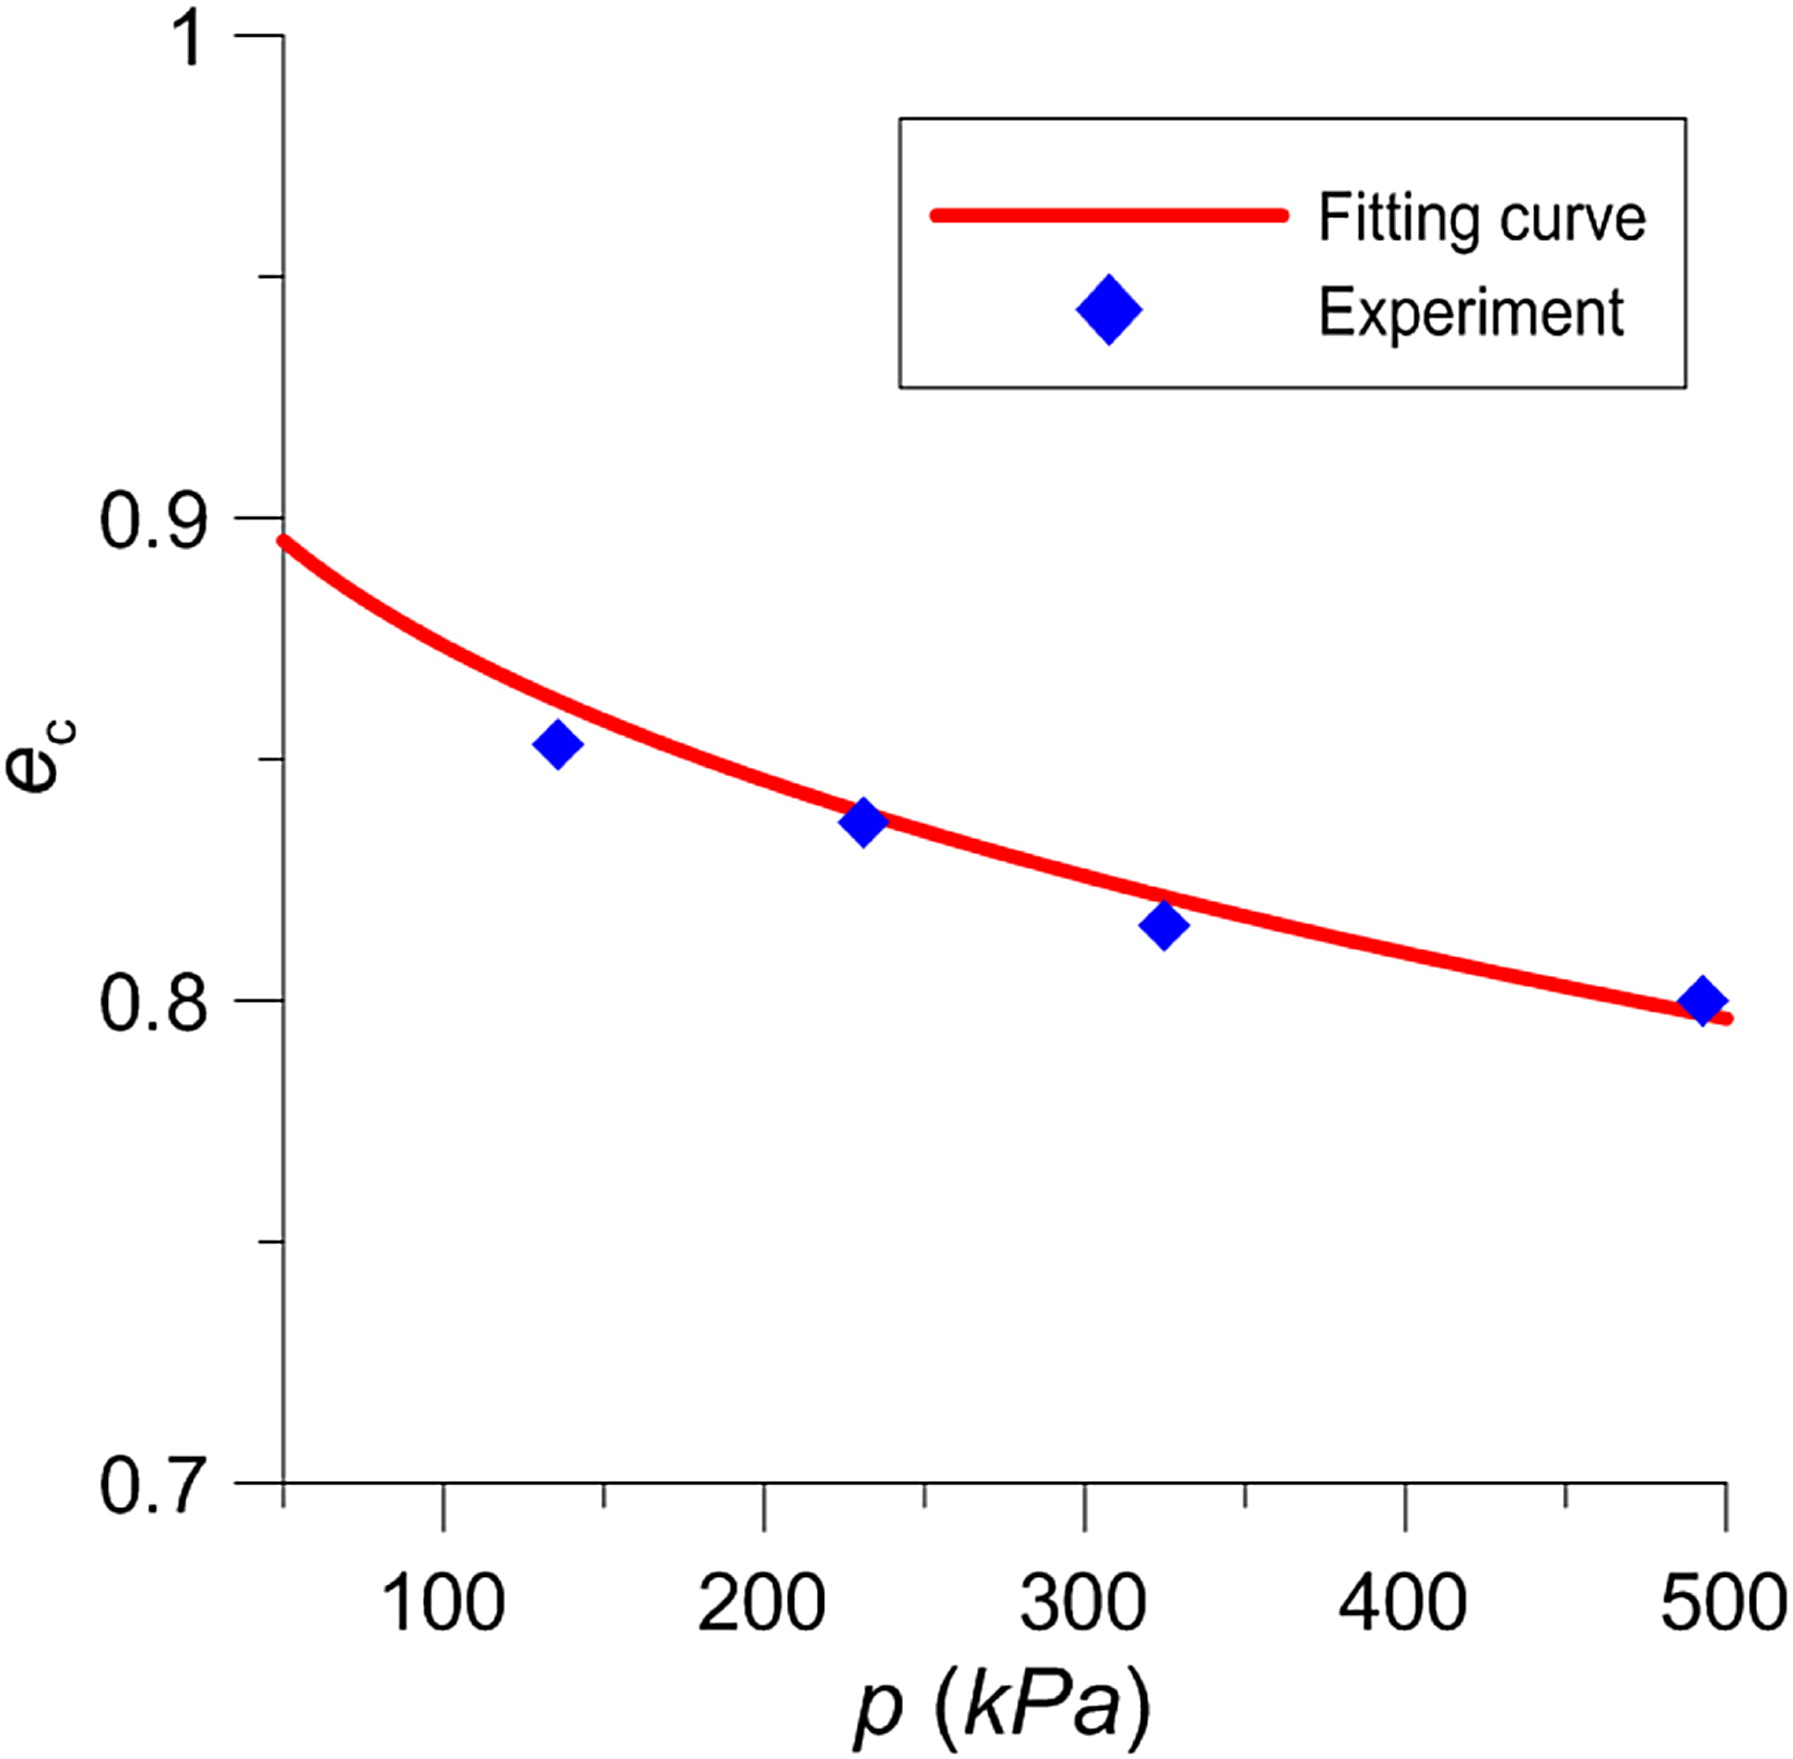
\includegraphics[width=.8\textwidth]{figures/figure8.jpg}
            \bicaption{The $e_c-p$ curve at critical state (experimental data from \citet{Chu2003})}{临界状态下的$e_c-p$曲线(实验数据来自\citealt{Chu2003})}
            \label{figure:8}
        \end{figure}
        \begin{figure}[H]
            \centering
            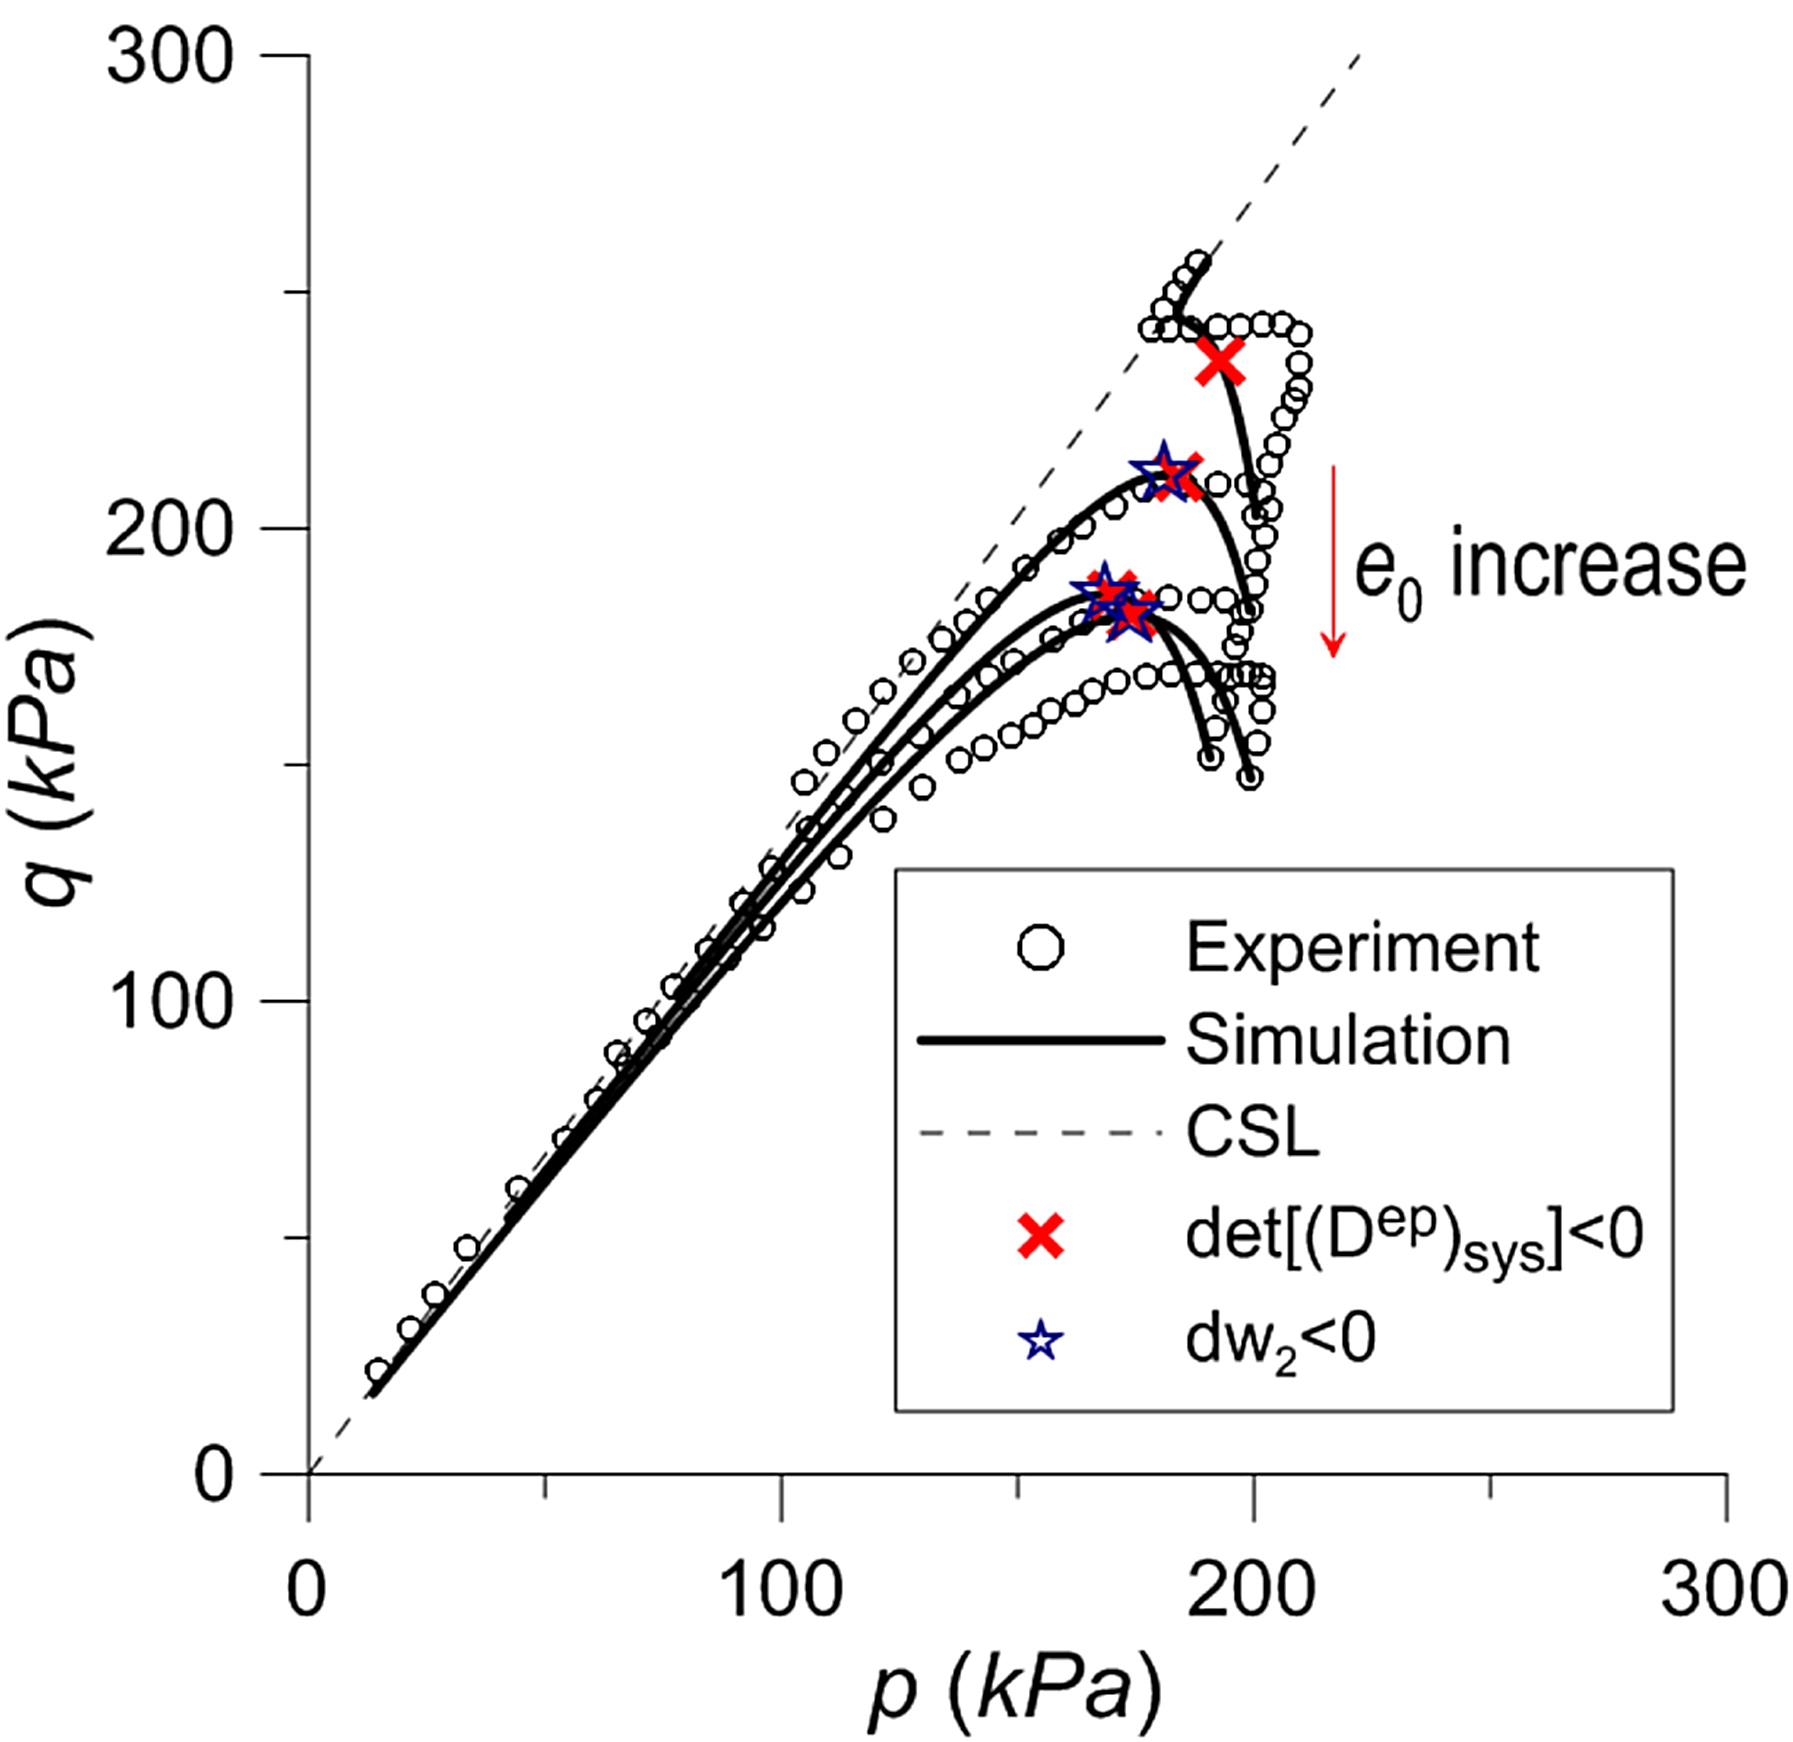
\includegraphics[width=.8\textwidth]{figures/figure9.jpg}
            \bicaption{Stress path of  $K_0$-consolidated undrained triaxial test (experimental data from \citealt{Chu2008})}{$K_0$固结三轴不排水试验的应力路径(实验数据来自\citealt{Chu2008})}
            \label{figure:9}
        \end{figure}
    \end{minipage}
    \hspace{0.02\textwidth}
    \begin{minipage}[b]{.48\textwidth}
        \begin{figure}[H]
            \centering
            \subfigure[stress-strain relationship 应力应变关系]{
                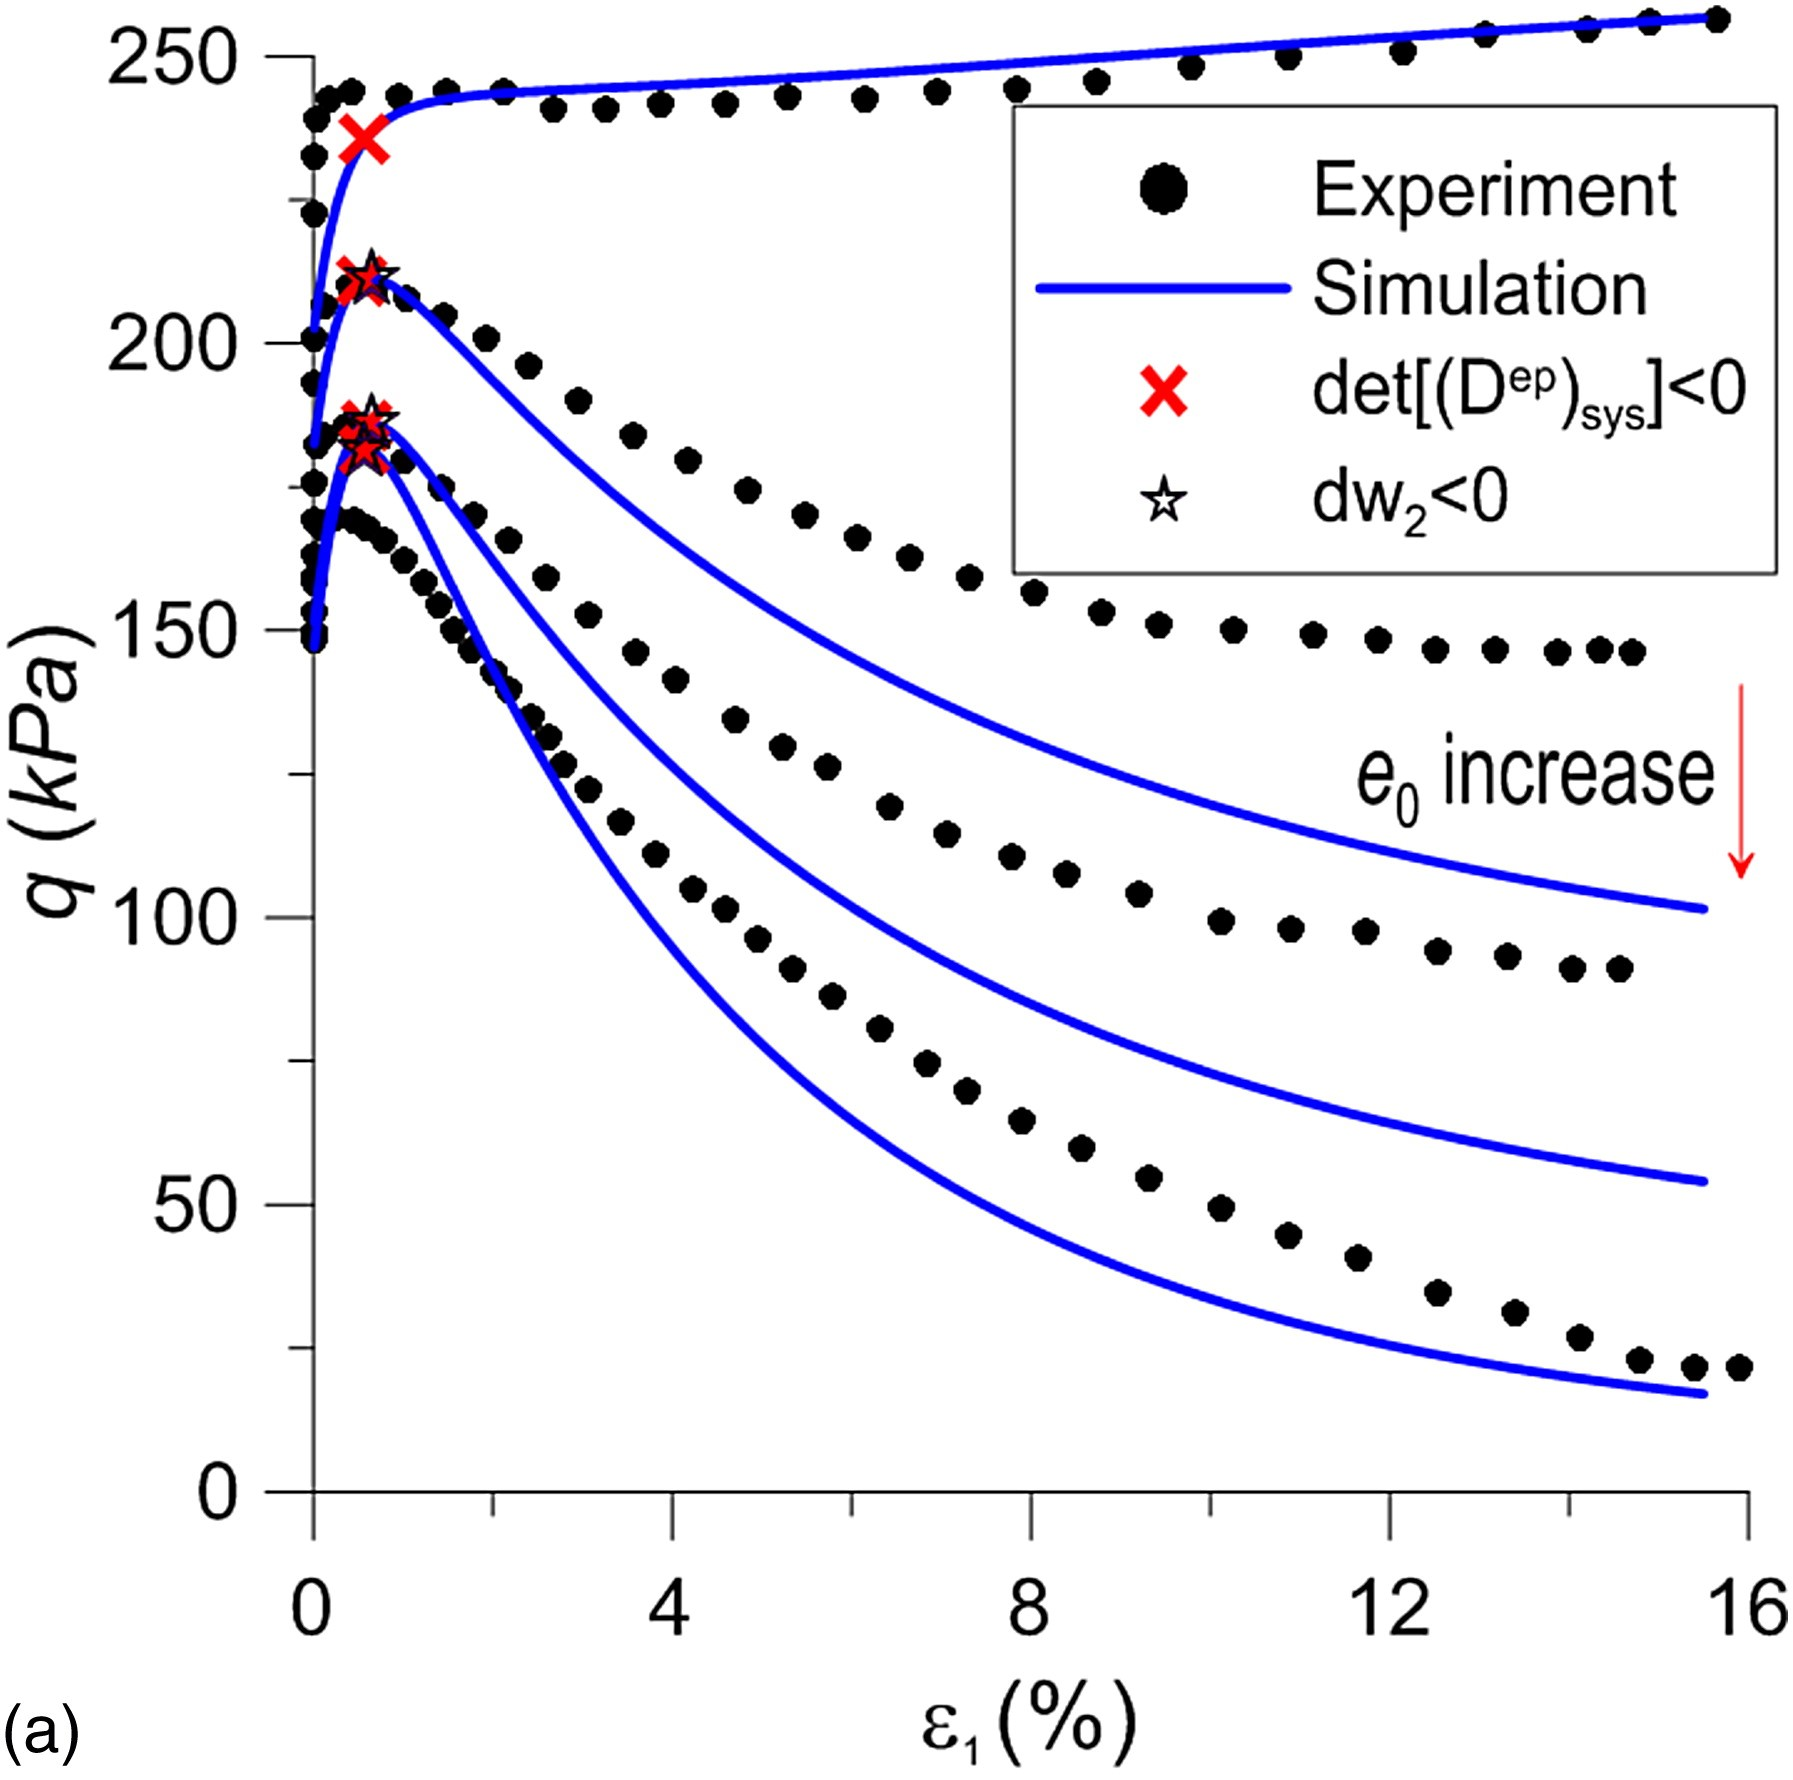
\includegraphics[width=.8\textwidth]{figures/figure10a.jpg}
                \label{figure:10a}
            }
            \subfigure[evolution of pore-water pressure 孔隙水压力的演变]{
                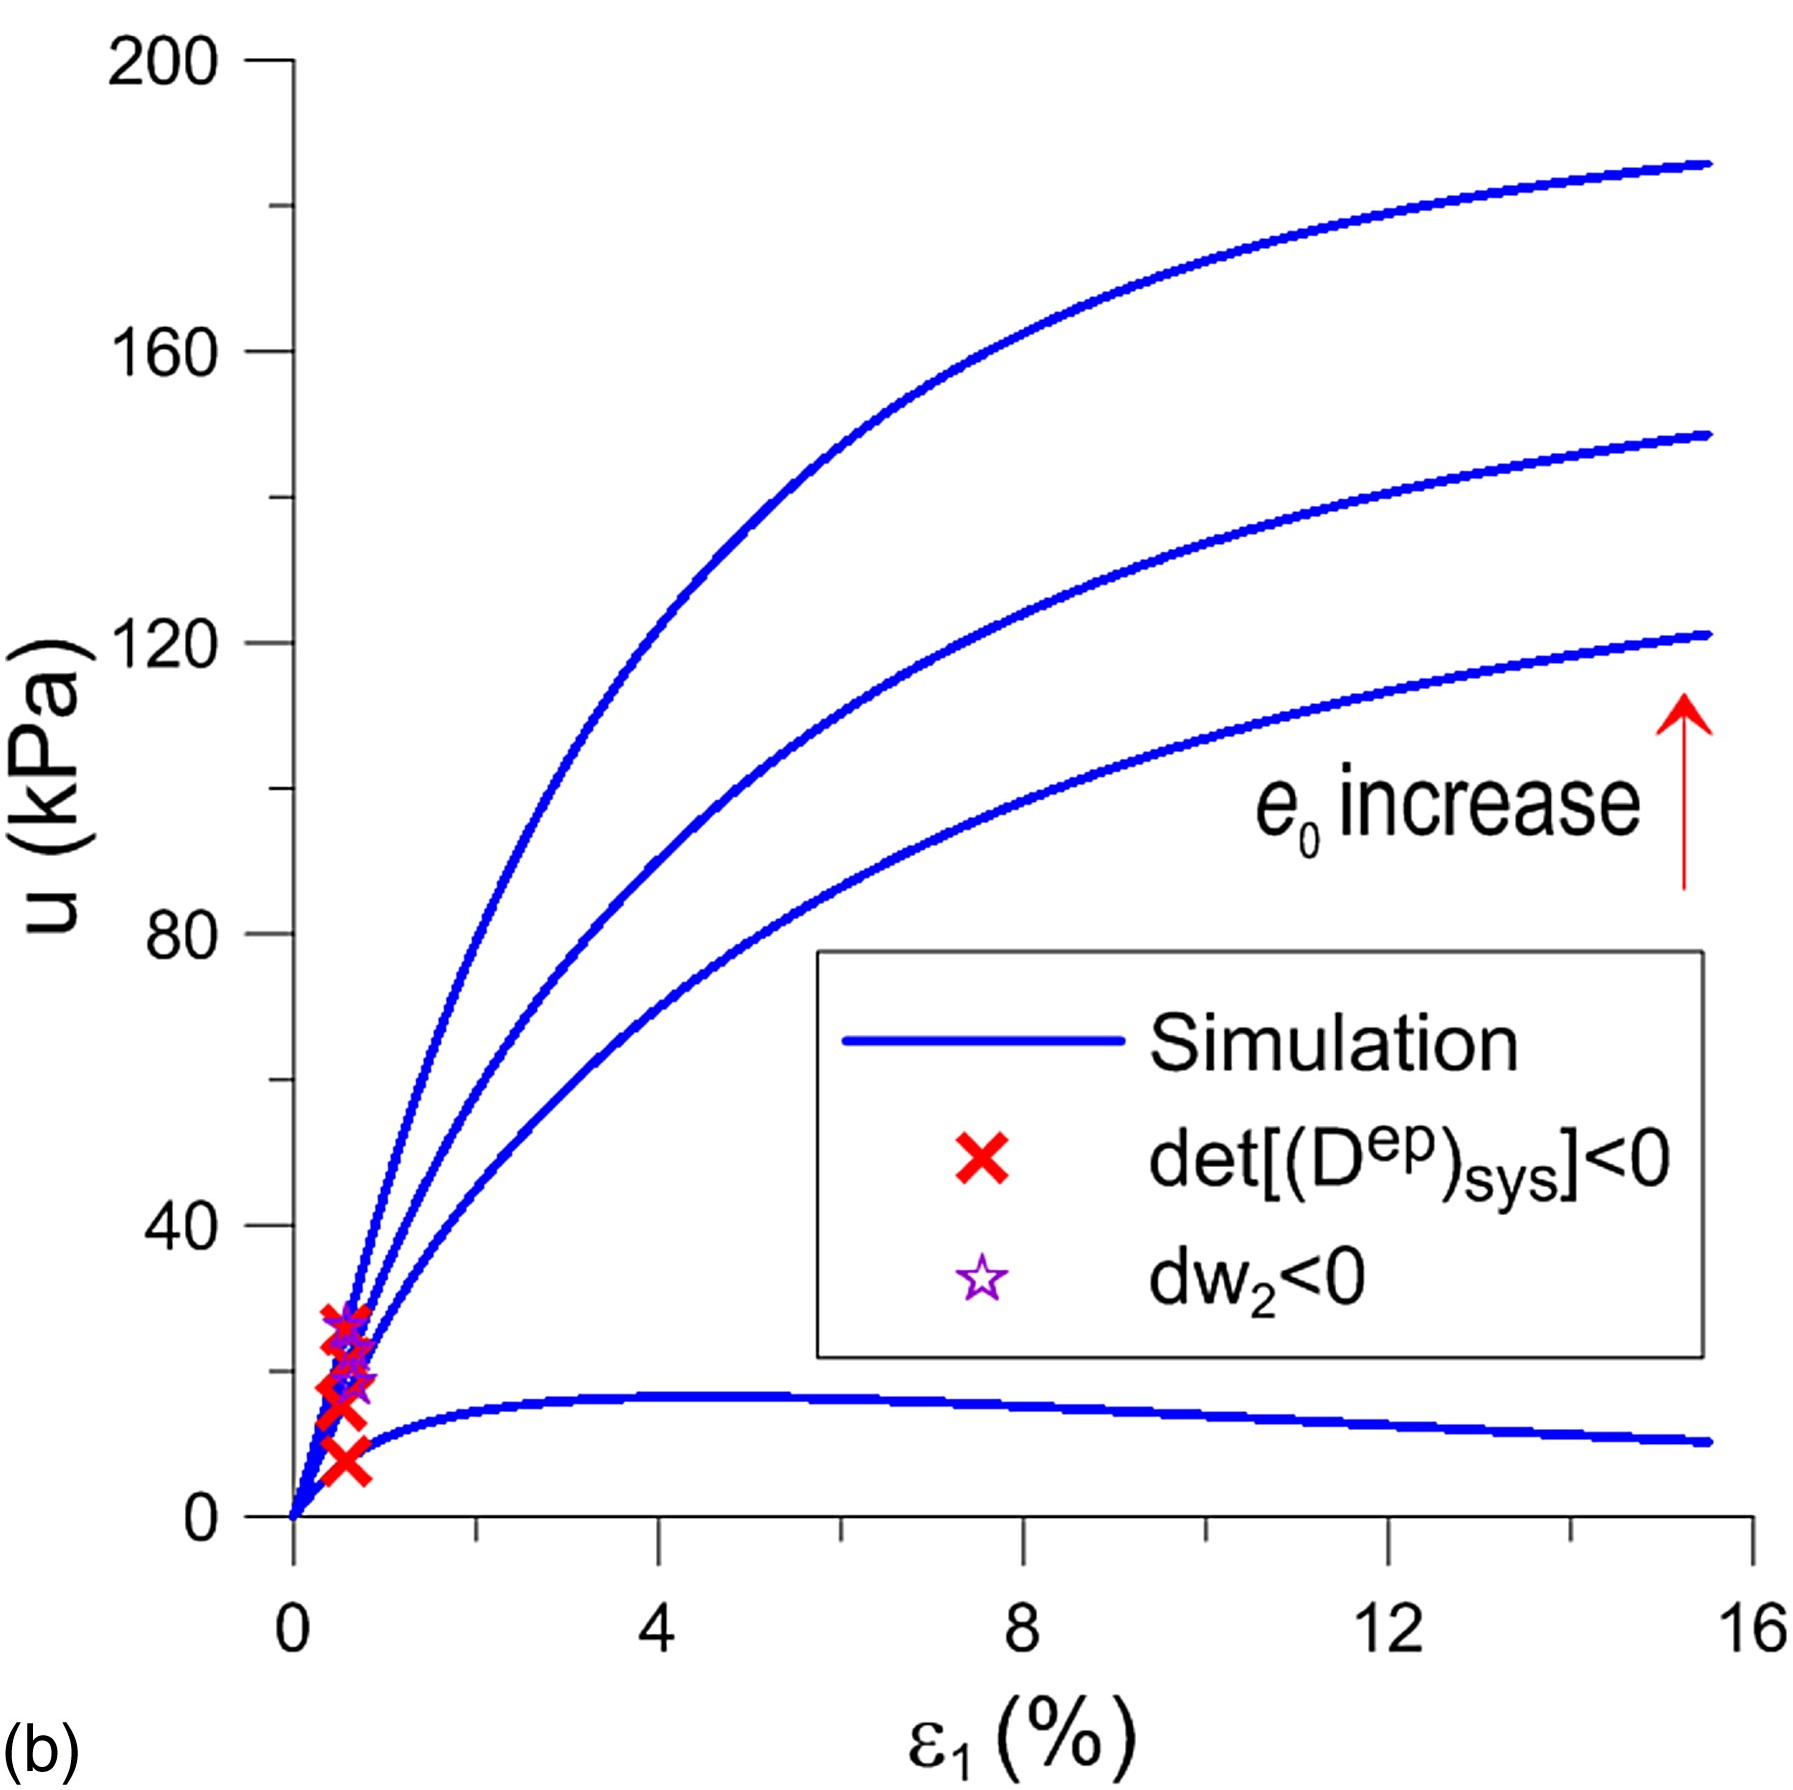
\includegraphics[width=.8\textwidth]{figures/figure10b.jpg}
                \label{figure:10b}
            }
            \bicaption{Model prediction (experimental data after Chu and \citealt{Chu2008})}{模型预测(来自\citealt{Chu2008}之后的实验数据)}
            \label{figure:10}
        \end{figure}
    \end{minipage}
\end{figure}
    }
    \switchcolumn*[\bisubsection*{$K_0$-Consolidated Undrained Triaxial Tests}{$K_0$三轴固结不排水试验}]

    The proposed constitutive model and instability criteria were used to predict the results of the $K_0$-consolidated undrained triaxial tests of \citet{Chu2008}. The specimen was made of Singapore marine-dredged silica sand with mean grain size 0.30–0.35 mm, uniformity coefficient 2.0, specific gravity 2.6, maximum void ratio 0.916, and minimum void ratio 0.533. The specimen was 100 mm in diameter and 190 mm in height. After $K_0$ consolidation, the void ratios of the specimens were 0.844, 0.881, 0.899, and 0.922.

    \switchcolumn

    所提出的本构模型和不稳定性标准被用于预测\citet{Chu2008}的$K_0$三轴固结不排水试验的结果。 样品由新加坡海洋挖出的硅砂制成,平均粒度为0.30–0.35毫米,不均匀系数为2.0,比重为2.6,最大孔隙比为0.916,最小孔隙比为0.533。 样品的直径为100毫米,高度为190毫米。 $K_0$固结后,样品的孔隙比分别为0.844、0.881、0.899和0.922。

    \switchcolumn*

    As shown in \enautoref{figure:8}, the $e_c-p$ curve at the critical state was calibrated from the experimental results of \citet{Chu2003} in the same sands. By using the material parameters in \enautoref{table:1}, the mechanical behavior of the $K_0$-consolidated saturated sands under undrained loading were obtained. The predicted effective stress path is shown in \enautoref{figure:9}. For relatively loose sand ($e_0 = 0.881,0.899,0.922$), the undrained loading induced the reduction of the mean pressure and the increase of deviatoric shear stress; after the attainment of its peak value, the deviatoric shear stress decreased. The test of the densest sands ($e_0 = 0.844$) showed the same trend as with the other three tests at the beginning of the loading stage; when the stress state approached the steady state, the deviatoric shear stress reversed and kept increasing, owing to the phase transition \citep{Ishihara1993}. The predicted stress-strain relationship and pore-water pressure are shown in Figs. \ref{figure:10a} and \ref{figure:10b}. The deviatoric shear stress first increased and then decreased with the applied strain in three relatively loose sand specimens; in the case of the densest sand specimen, the deviatoric shear stress kept increasing and the peak value never appeared. As shown in \enautoref{figure:10b}, the pore-water pressure increased to a constant value when the sands reached the steady state. Compared with the three looser specimens, less pore-water pressure developed in the relatively dense specimen.

    \switchcolumn

    如 \cnautoref{figure:8} 所示,根据 \citet{Chu2003} 在相同砂土中的实验结果,对临界状态下的$e_c-p$曲线进行了校准。通过使用 \cnautoref{table:1} 中的材料参数,获得了在不排水的情况下$K_0$固结的饱和砂土的力学行为。预测的有效应力路径如\cnautoref{figure:9}所示。对于相对疏松的砂土($e_0 = 0.881,0.899,0.922$),不排水的载荷引起平均压力的降低和偏剪应力的增加。达到峰值后,偏剪应力减小。在加载阶段开始时,最稠密的砂的试验($e_0 = 0.844$)显示出与其他三个试验相同的趋势。当应力状态接近稳态时,由于发生了相变,偏剪应力逆转并持续增加 \citep{Ishihara1993}。预测的应力应变关系和孔隙水压力如 \cnautoref{figure:10a} 和 \cnautoref{figure:10b} 所示。在三个相对松散的砂岩样品中,随施加的应变,偏向剪切应力首先增大,然后减小。在最稠密的砂土样品中,偏剪应力不断增加,并且从未出现峰值。如 \cnautoref{figure:10b} 所示,当砂达到稳态时,孔隙水压力增加到一个恒定值。与三个较松散的样品相比,在相对致密的样品中产生的孔隙水压力较小。

    \switchcolumn*

    The determinant of the symmetric part of elastoplastic modulus tensor [\enautoref{figure:11a}] and the second-order work [\enautoref{figure:11b}] were calculated; all the determinants became negative when loading to approximately $0.6\%$ of axial strain, which indicates that all the samples entered into potentially unstable states. As shown in \enautoref{figure:11b}, the second-order work for the densest specimen ($e_0=0.844$) never turned negative, which indicates that static liquefaction would not occur. As shown in \enautoref{figure:12}, although the stresses showed a descending trend after the onset of static liquefaction, both the potentially unstable points and static liquefaction point occurred at the hardening regime. To clarify the influence of the initial material state on the shear strength at static liquefaction, the relationship between the initial void ratio and the stress ratio at the instability point is shown in \enautoref{figure:12}. The stress ratio at the instability point decreased along with the increase of initial void ratio, and the predicted results agreed with the experimental results.

    \switchcolumn

    计算弹塑性模量张量(\cnautoref{figure:11a})的对称部分和二次功(\cnautoref{figure:11b})的行列式;当加载到轴向应变的大约$0.6\%$时,所有决定因素都变为负值,这表明所有样本都进入了潜在的不稳定状态。如\cnautoref{figure:11b}所示,最稠密样品($e_0 = 0.844$)的二阶功从未变为负值,这表明不会发生静态液化。如\cnautoref{figure:12}所示,尽管在静态液化开始后应力显示出下降的趋势,但潜在的不稳定点和静态液化点都发生在硬化区。为了阐明初始材料状态对静态液化时抗剪强度的影响,初始孔隙率与不稳定性点处的应力比之间的关系如\cnautoref{figure:3}所示。不稳定性点处的应力比随着增加而减小初始空隙率的计算结果与实验结果吻合。

    \CrossColumnText{
        \begin{figure}[p]
    \centering
    \begin{minipage}[b]{.48\textwidth}
        \begin{figure}[H]
            \centering
            \subfigure[determinant of the symmetric part of the elastoplastic modulus tensor 弹塑性模量张量的对称部分的行列式的演变]{
                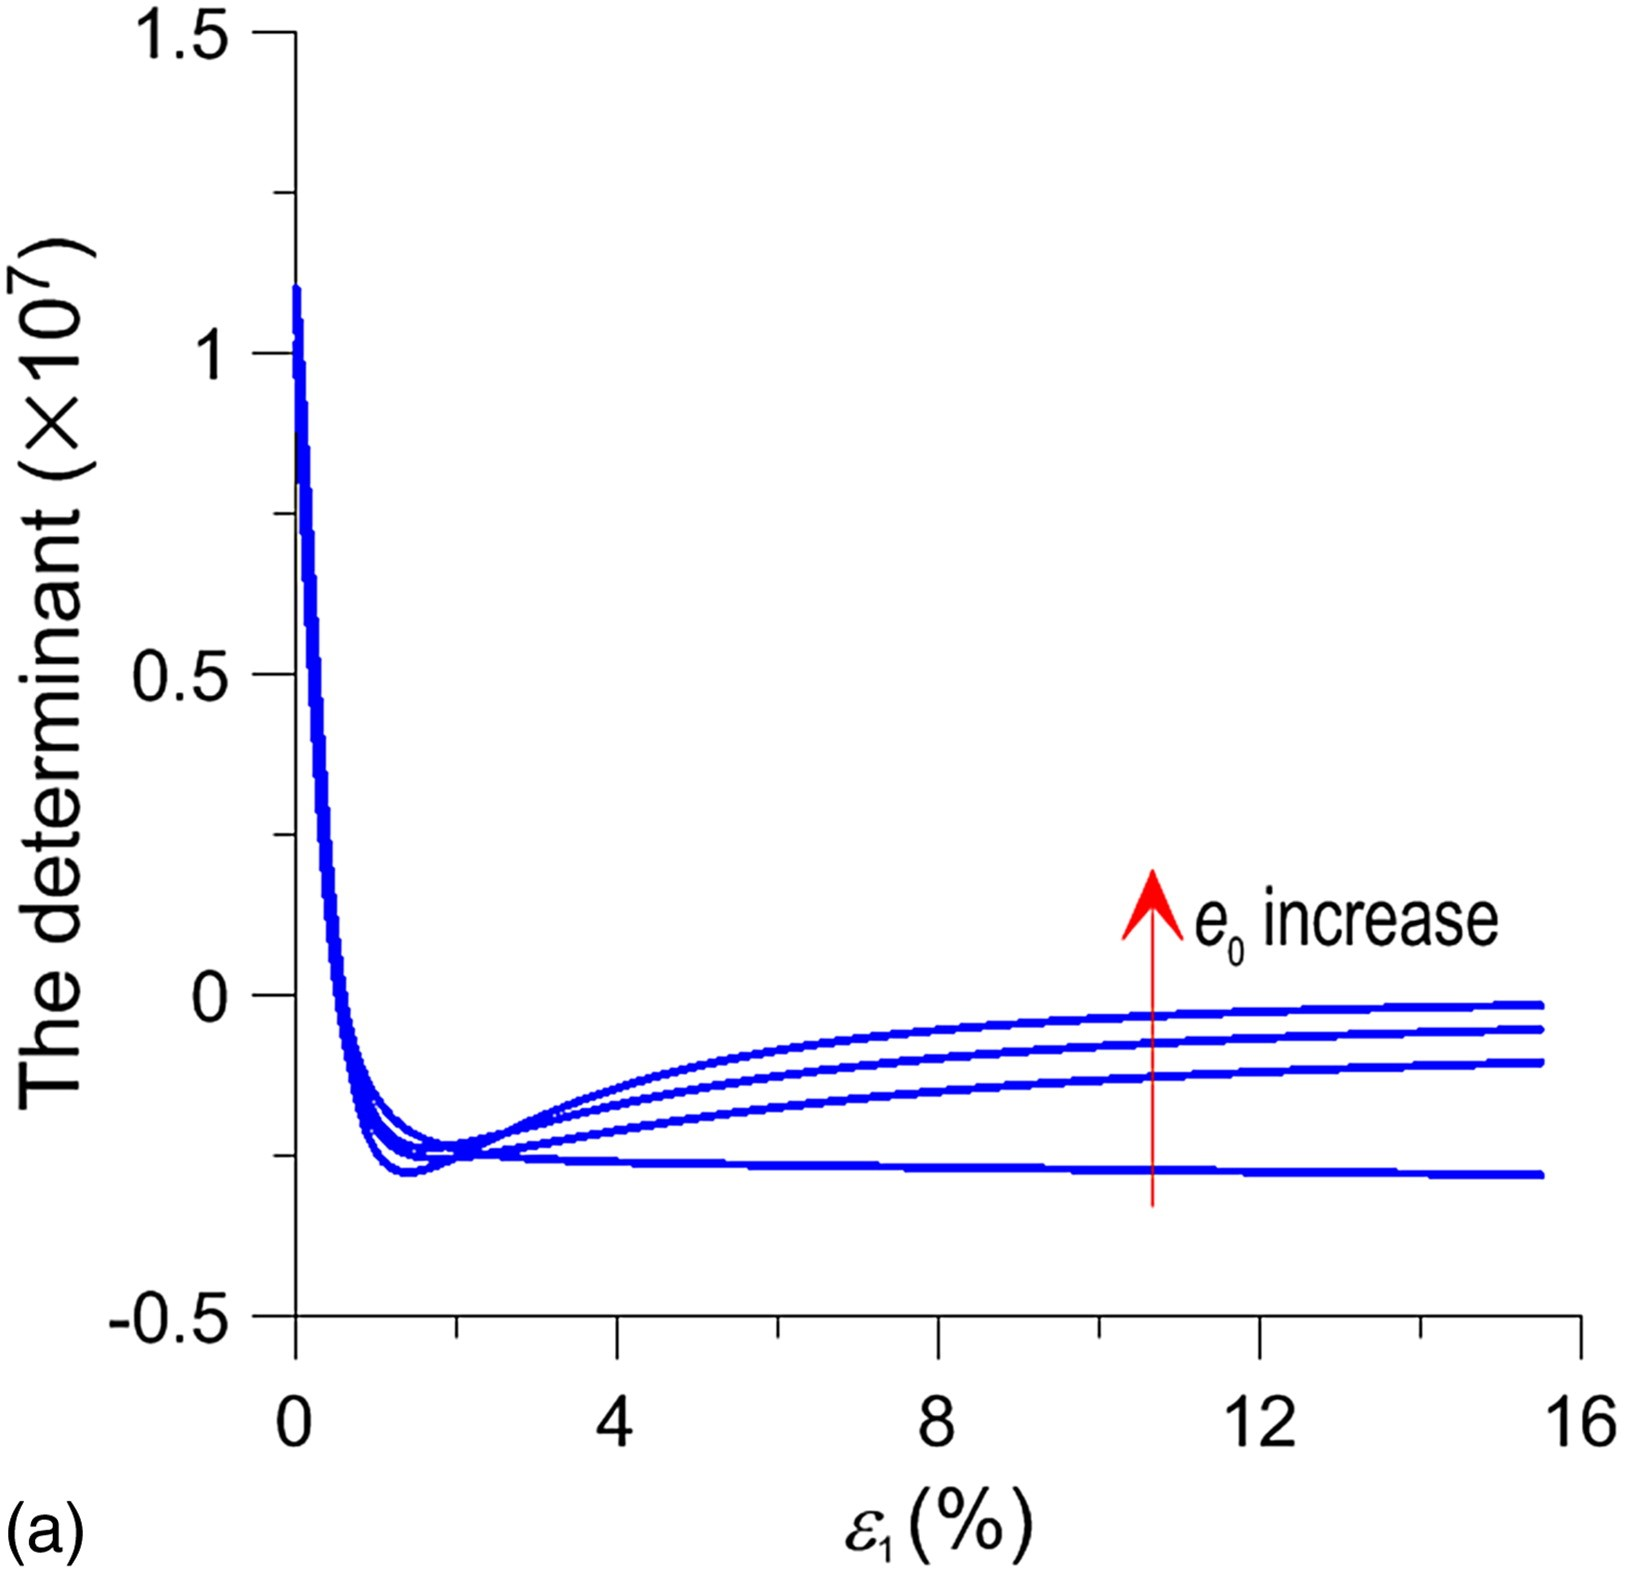
\includegraphics[width=\textwidth]{figures/figure11a.jpg}
                \label{figure:11a}
            }
            \subfigure[evolution of second-order work 二阶功]{
                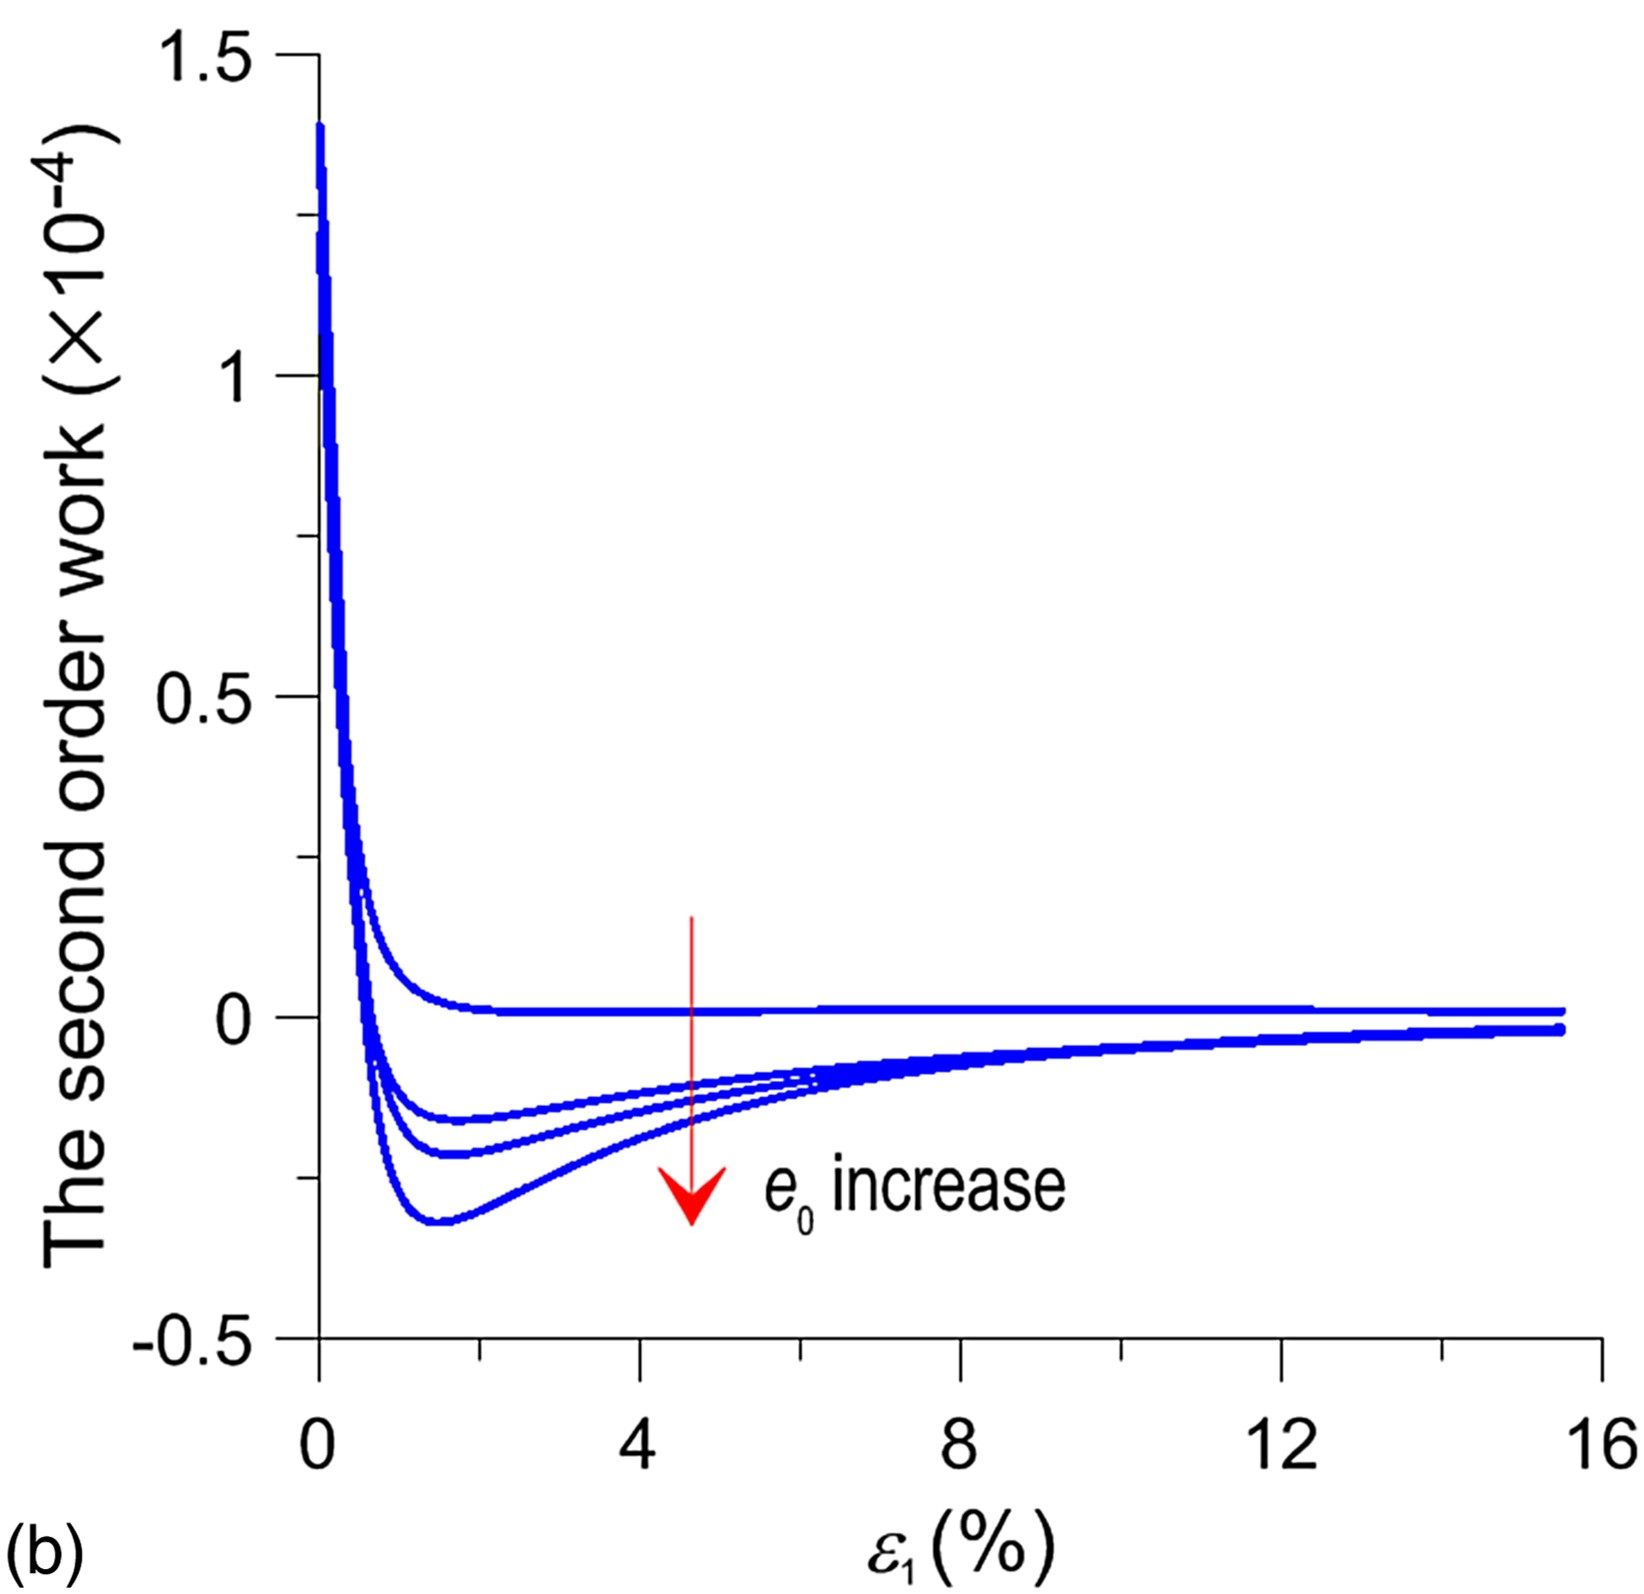
\includegraphics[width=\textwidth]{figures/figure11b.jpg}
                \label{figure:11b}
            }
            \bicaption{Evolution of determinant of the symmetric part of the elastoplastic modulus tensor and second-order work}{弹塑性模量张量的对称部分的行列式的和二阶功的演变}
            \label{figure:11}
        \end{figure}
    \end{minipage}
    \hspace{0.02\textwidth}
    \begin{minipage}[b]{.48\textwidth}
        \begin{figure}[H]
            \centering
            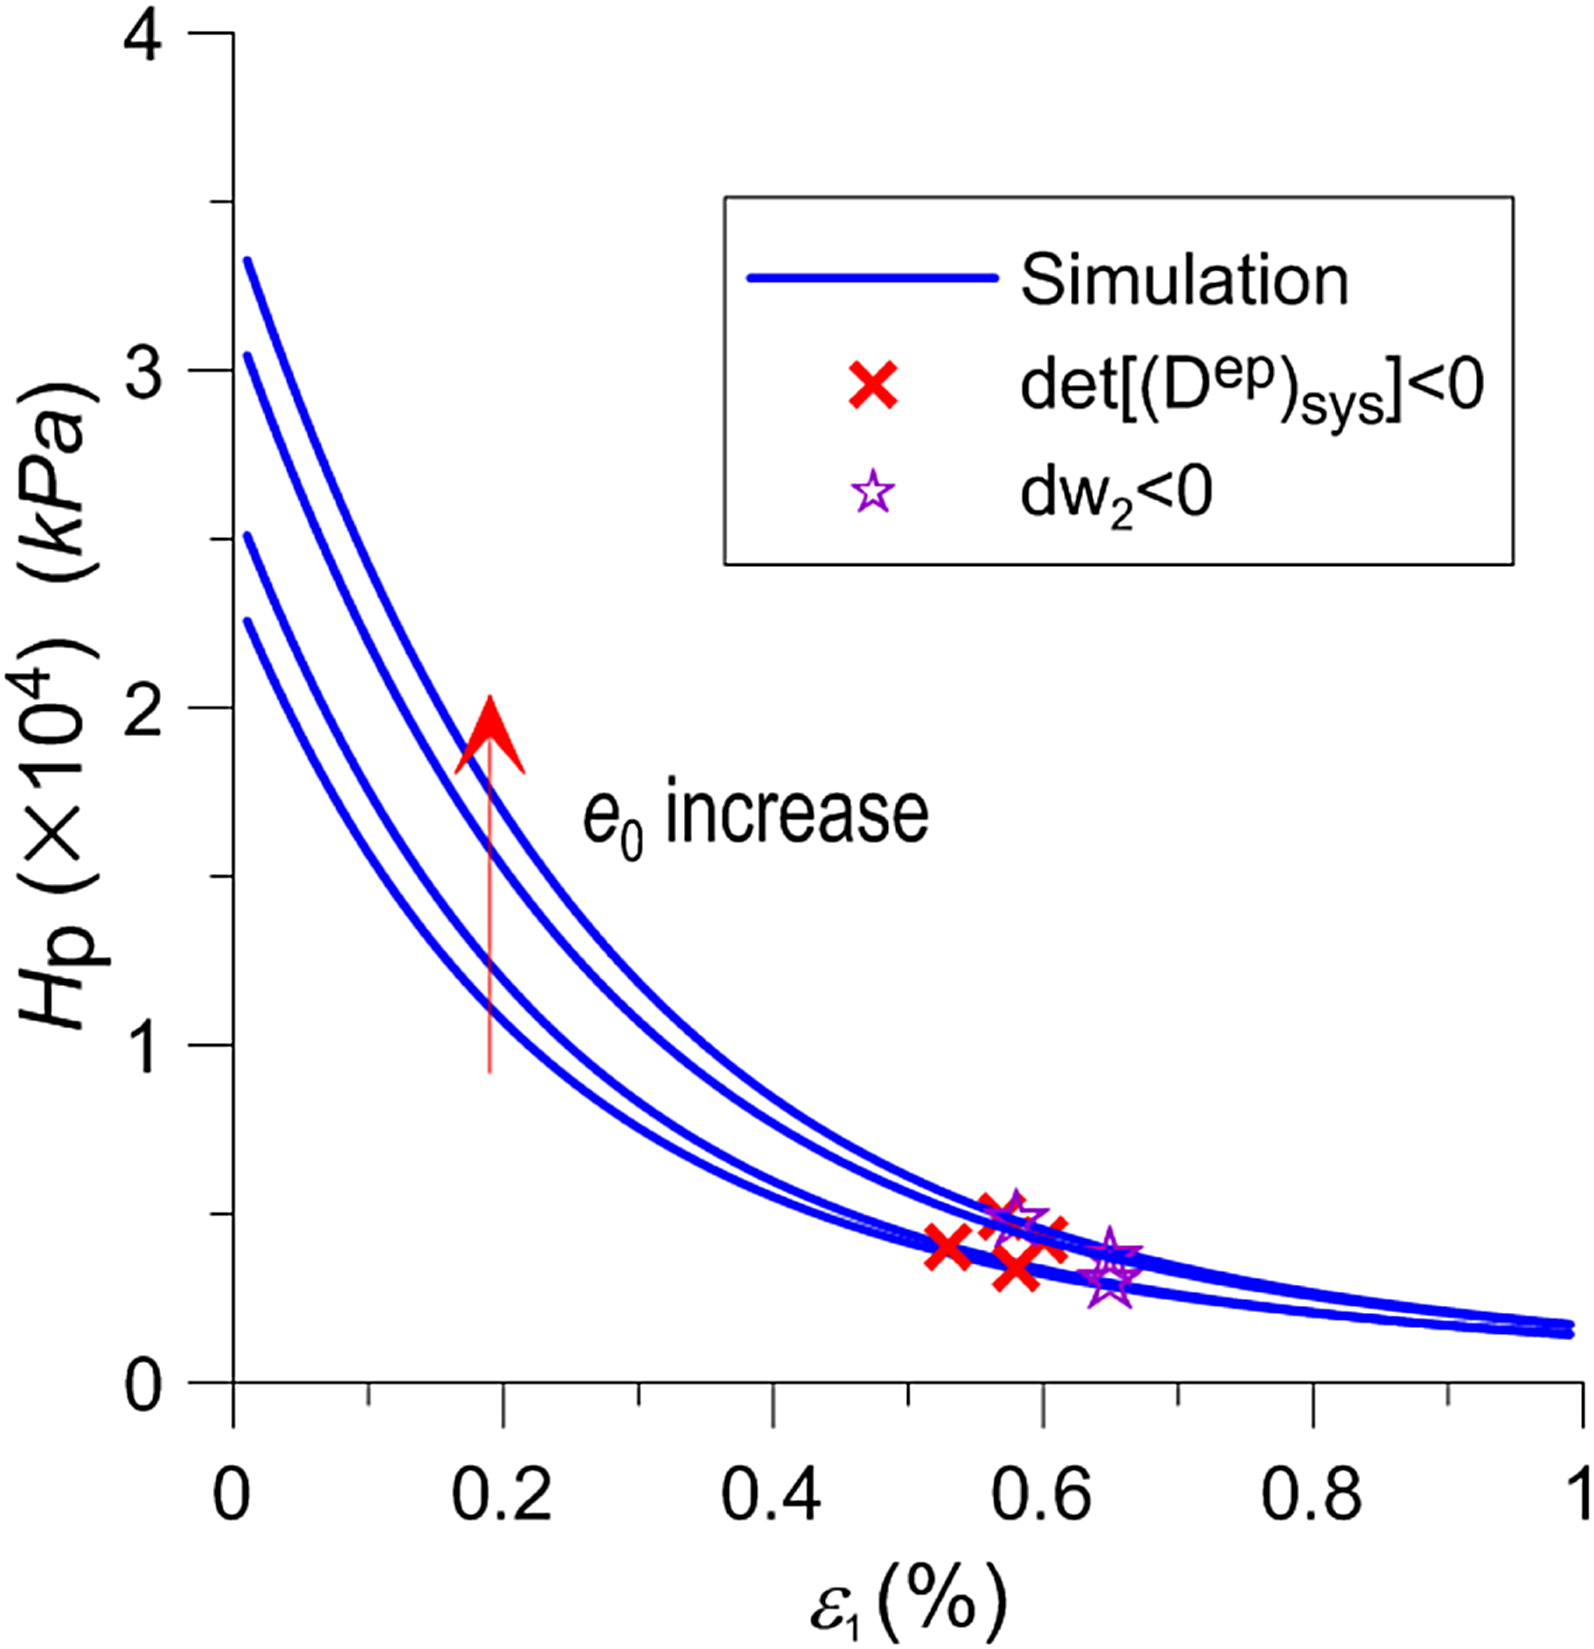
\includegraphics[width=\textwidth]{figures/figure12.jpg}
            \bicaption{Evolution of hardening modulus}{硬化模量的演变}
            \label{figure:12}
        \end{figure}
        \begin{figure}[H]
            \centering
            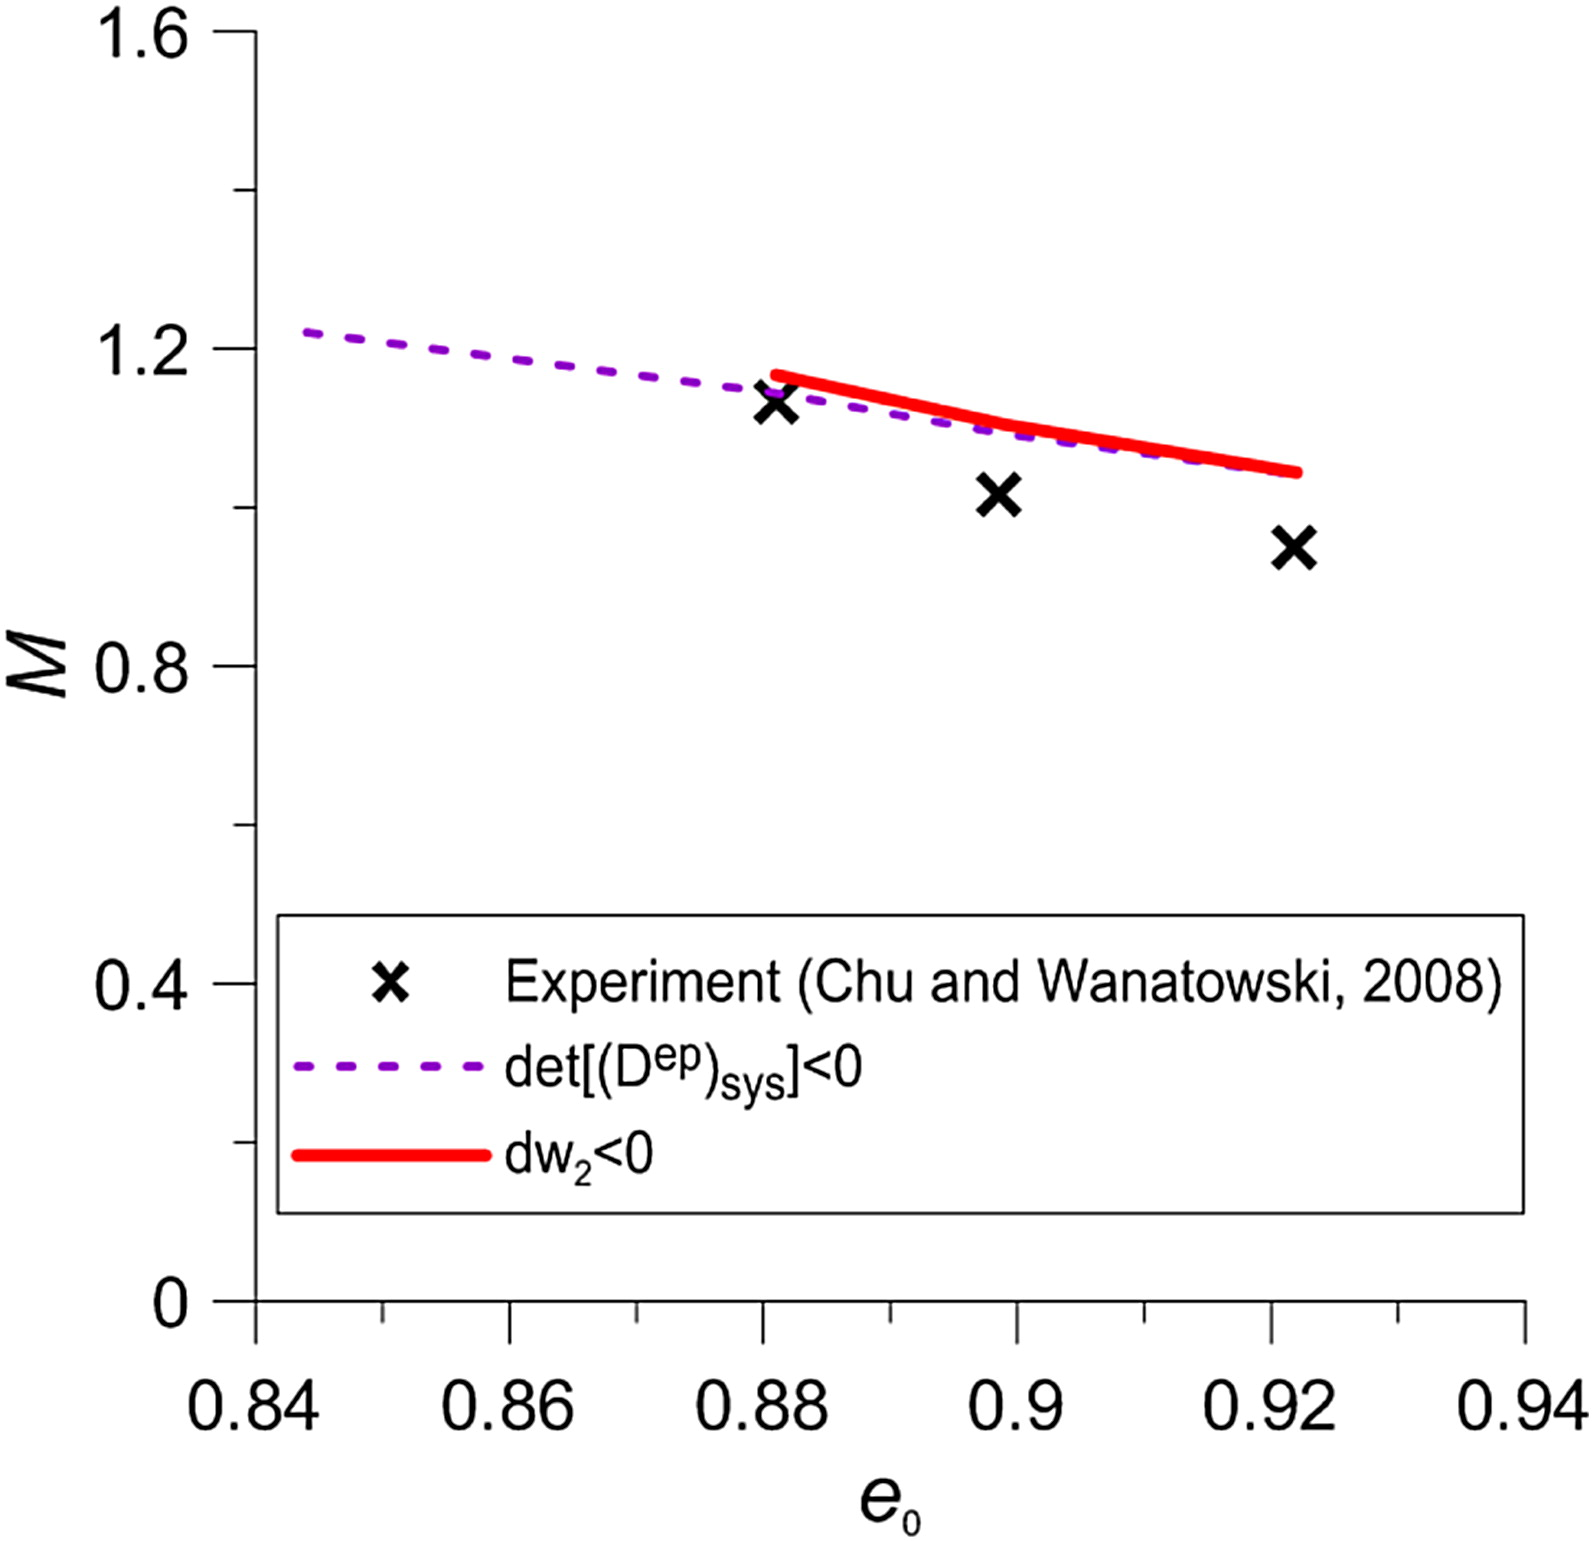
\includegraphics[width=\textwidth]{figures/figure13.jpg}
            \bicaption{Influence of the initial void ratio on the stress ratio at the onset of static liquefaction}{初始液化比对静态液化开始时应力比的影响}
            \label{figure:13}
        \end{figure}
    \end{minipage}
\end{figure}
    }

\end{ParaColumn}
\begin{ParaColumn}[\bisection*{Conclusions}{结论}]

    A state-dependent nonassociated Mohr-Coulomb hardening elastoplasticity model and second-order work criterion were proposed to study the static liquefaction under the undrained triaxial condition. The vanishing value of the determinant of the symmetric part of the elastoplastic modulus tensor was used to predict the potentially unstable state of soils, and the sign change in second-order work denoted the onset of static liquefaction. The static liquefaction initiated only when the undrained stress path occurred along with the potentially unstable stress path, or when the soil stayed stable even the stress state was located in the potentially unstable region.

    \switchcolumn

    为了研究在不排水的三轴条件下的静态液化,提出了一种状态相关的非关联摩尔库伦硬化弹塑性模型和二阶功准则。 弹塑性模量张量的对称部分的行列式值用于预测土体的潜在不稳定状态,并且二阶功的符号变化表示静态液化的开始。 静态液化仅在不排水的应力路径与潜在的不稳定应力路径同时发生时发生,或者当土体保持稳定甚至应力状态位于潜在不稳定区域时才开始。

    \switchcolumn*

    The proposed model and instability criteria were used to analyze a series of isotropically consolidated and $K_0$-consolidated undrained triaxial tests. The results showed that static liquefaction is prone to occur in loose sands, although when the sand is dense enough, it would be prevented by the tendency of dilatancy even if the state of sands becomes potentially unstable. The static liquefaction occurred at the hardening regime of sands before the plastic limit failure criterion was reached; its occurrence induced the drop of shear resistance and the increase of pore-water pressure.

    \switchcolumn

    采用所提出的模型和失稳准则进行了一系列的等向固结和$K_0$固结不排水三轴试验。结果表明:松散砂土容易发生静态液化,但当砂土密实度足够大时,即使砂土的状态变得潜在不稳定,其膨胀趋势也会阻止静态液化的发生。静力液化发生在砂体硬化区,未达到塑性极限破坏准则;其发生导致剪切阻力下降,孔隙水压力增大。
\end{ParaColumn}
\begin{ParaColumn}[\bisection*{Acknowledgments}{致谢}]
    
    The financial support given by the National Basic Research Program of China (grant 2012CB719803), National Science Foundation of China (NSFC grant 11372228), and Shanghai Municipal Science and Technology Commission (grant 13ZR1443800) are gratefully acknowledged. The first author also extends his thanks to Professor José E Andrade at the California Institute of Technology for his help in doing the research. The authors are grateful to the anonymous reviewers for their helpful comments and suggestions.

    \switchcolumn

    在此感谢中国国家基础研究计划(2012CB719803),国家科学基金(NSFC grant 11372228)和上海市科学技术委员会(grant 13ZR1443800)的资助。 第一作者还对加利福尼亚理工学院的JoséE Andrade教授在研究方面的帮助表示感谢。 作者感谢匿名审阅者的有益评论和建议。
\end{ParaColumn}

\bibliographystyle{plainnat}
\bibliography{Lu2014.bib}

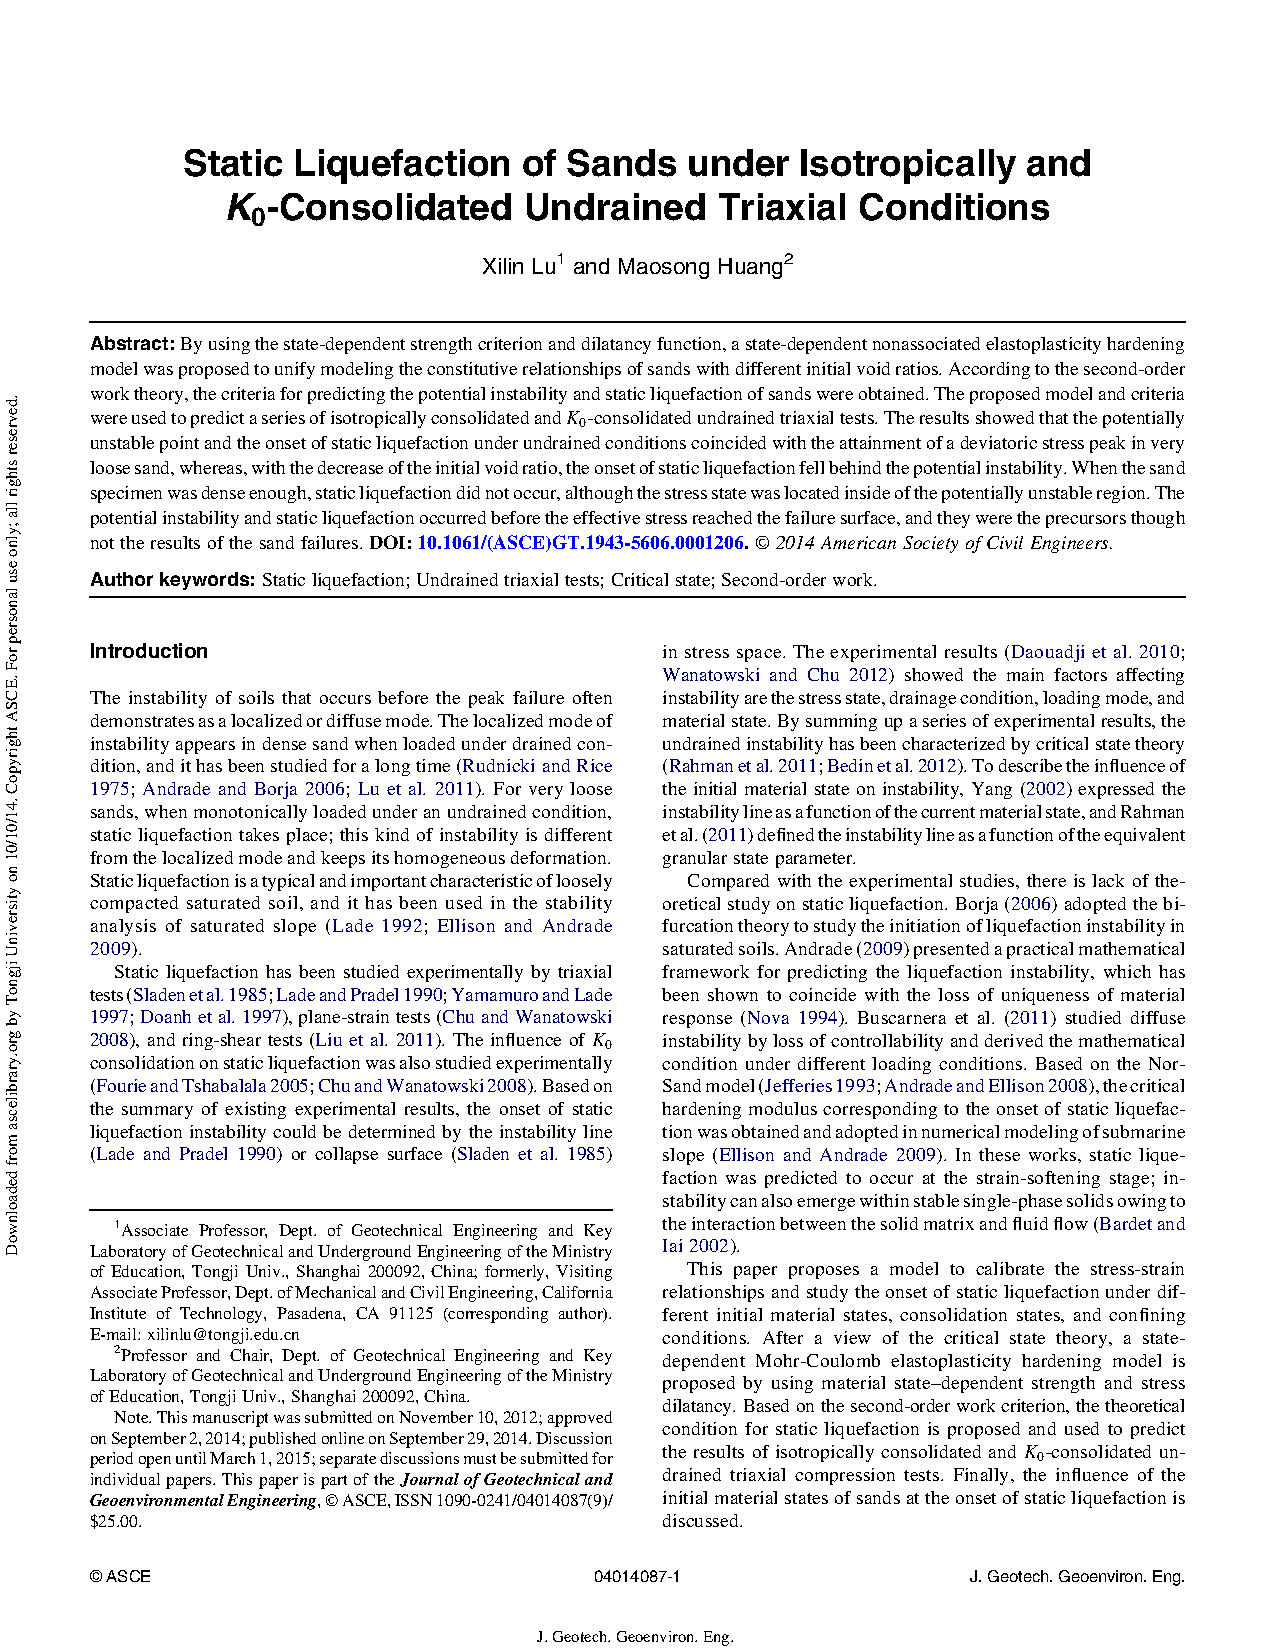
\includepdf[pages=1-9]{Static Liquefaction of Sands under Isotropically and K0-Consolidated Undrained Triaxial Conditions.pdf}
    
\end{document}